\documentclass[12pt,UTF8]{ctexbook}
\usepackage{ctex}
\usepackage{array}
\usepackage{graphicx}
\usepackage{wrapfig}
\usepackage[table,dvipsnames]{xcolor}
\usepackage{tabularx}
\usepackage{longtable}
\usepackage{float}
\usepackage{amsmath}
\usepackage{amssymb}
\usepackage{xfrac}
\usepackage{eucal}
\usepackage{titlesec}
\usepackage{amsthm}
\usepackage{tikz-cd}
\usepackage{enumitem}
\usepackage{verbatim}
\usepackage{fontspec,xunicode,xltxtra}
\usepackage{xeCJK} 
\usepackage{caption}
\usepackage{thmtools, thm-restate}
\usepackage{mhchem}
% 修改脚注的编号为加圈样式,并且各页单独编号
\usepackage{pifont}
\usepackage[b]{esvect}
\usepackage[perpage,symbol*]{footmisc}
\DefineFNsymbols{circled}{{\ding{192}}{\ding{193}}{\ding{194}}
{\ding{195}}{\ding{196}}{\ding{197}}{\ding{198}}{\ding{199}}{\ding{200}}{\ding{201}}}
\setfnsymbol{circled}

\definecolor{gl}{RGB}{246, 252, 240}
\definecolor{gd}{RGB}{236, 244, 230}
\definecolor{bg}{RGB}{242, 244, 228}

\setCJKmainfont[BoldFont=STZhongsong]{STSong}
\setCJKmonofont{simkai.ttf} % for \texttt
\setCJKsansfont{simfang.ttf} % for \textsf
\setlength\parskip{8pt}
\setlength{\fboxsep}{12pt}
\renewcommand\thesection{\arabic{chapter}.\arabic{section}}
\newcommand{\arccot}{\operatorname{arccot}}
\newcommand{\dlim}[1]{^{\color{gray}\prime}#1}
\newcommand{\lian}[1]{
    \underset{#1}{\operatorname{lian}\,}
}
\newcommand{\di}[1]{\,\mathrm{d}#1}
\newcommand{\qu}[2]{\displaystyle\left(#1;#2\right)}
% developpements limites
\newcommand{\oveq}[1]{\overset{#1}{=}} 
\newcommand{\olim}[1]{\mathit{o}\left(#1\right)}  % petit o
\newcommand{\Olim}[1]{\mathcal{O}\left(#1\right)}  % grand O
\newcommand{\Tlim}[1]{\mathcal{\Theta}\left(#1\right)}  % grand theta
\newcommand{\eqlim}[1]{\overset{#1}{\sim}}  % equivalence
\newcommand{\vect}[1]{\left\langle #1 \right\rangle}
\newcommand{\nji}[2]{\displaystyle\left( #1 \,|\, #2\right)}
\newcommand{\rectbx}{%
    \mathord{\text{%
        \tikz[baseline] \draw (0,.1ex) -- (.4em,.1ex) -- (.4em,1.5ex) -- (0em,1.5ex) -- cycle;}
    }
}

\theoremstyle{definition}
\newtheorem{df}{定义}[section] 
\newtheorem*{po}{公理}
\newtheorem{pp}{命题}[section]
\newtheorem{tm}{定理}[section]
\newtheorem{cor}{推论}[pp]
\newtheorem{ex}{例子}[section]
\newtheorem{et}{例题}[section]
\newtheorem*{ex*}{例子}
\newtheorem*{so}{解答}
\theoremstyle{plain}
\newtheorem{sk}{思考}[section]
\newtheorem{xt}{习题}[section]
\renewenvironment{proof}{\paragraph{\textbf{证明:}}}{\hfill$\square$}

% 列举环境的行间距
\setenumerate[1]{itemsep=0pt,partopsep=0pt,parsep=0pt,topsep=0pt}
\setitemize[1]{itemsep=0pt,partopsep=0pt,parsep=0pt,topsep=0pt}
\setdescription{itemsep=0pt,partopsep=0pt,parsep=0pt,topsep=0pt}
% 章节字体大小
\titleformat{\section}{\zihao{-2}\bfseries}{ \thesection }{16pt}{}
% 封面
\title{\zihao{0} \bfseries 第五册}
\author{\zihao{2} \texttt{大青花鱼}}
% \date{\bfseries\today}
\date{}
% 正文
\begin{document}
\maketitle
\tableofcontents
\newpage

\chapter{度量和度量以外}

数学的重要研究对象之一,就是平面、立体空间中的形状。我们从中抽象出了平面形和空间形,定义了点、直线、曲线、平面、三角形、圆形等概念,
通过距离、长度、角度来描述、理解它们的性质。我们构造了向量和平直空间、直变换的概念,来描述、理解平面形、空间体的变化。

另一方面,我们通过研究实变量的函数,对平面中的曲线有了一定了解。通过研究连续函数及其微变率的性质,
我们对作为函数图像的曲线有了基本认识。为了更好地理解平面乃至空间中的形状,我们需要更多的工具。

我们把空间视为点的集合。向量就是描述这些点和空间关系的一种方法。我们通过内积定义了向量的距离、长度、角度,从而可以描述空间中的形状。
我们把这样的空间称为内积空间(即配备了内积的空间)。空间形作为点的集合,可以用距离、长度、角度来描述。

我们把和距离、长度、角度相关的性质称为\textbf{度量性质}。除此之外,平面形、空间体作为点的集合,还有其他的性质。
比如,我们讨论函数图像的性质的时候,往往讨论“一点附近”或“无穷远处”的行为。这些概念和具体的长度、距离关系不大。
这些性质对我们理解空间形状的本质十分重要。

\section{邻域、开集和闭集}

为了理解数轴上的点集,我们引进了区间的概念。区间是一种基本的点集。为了研究曲线在一点附近的情况,我们引入了邻域的概念。
邻域可以用来方便地描述“附近”这件事。对于平面上乃至空间中的点集,我们也引入一些基本的概念,帮助我们描述定义在平面和空间上的映射。

从数轴上的区间的概念出发,我们可以定义平面乃至空间上的“区间”:

\begin{df}{\textbf{方区}}
    给定开区间$(a;b)$、$(c;d)$\footnote{其中$a,b,c,d$可以为无穷大。},我们称平面点集:
    $$\{(x, y) \, | \, a < x < b,\, c< x < d\}$$
    为$(a;b)$、$(c;d)$构成的\textbf{开方区},记为$(a;b)\times(c;d)$。

    给定闭区间$[a;b]$、$[c;d]$,我们称平面点集:
    $$\{(x, y) \, | \, a \leqslant x \leqslant b,\, c \leqslant x \leqslant d\}$$
    为$[a;b]$、$[c;d]$构成的\textbf{闭方区},记为$[a;b]\times[c;d]$。

    一般来说,如果有数$a,b,c,d$使得平面点集$S$满足:
    $$(a;b)\times(c;d) \subseteq S \subseteq [a;b]\times[c;d],$$
    就说$S$是$a,b,c,d$构成的方区,记为$\rectbx_{a;b;c;d}$。

\end{df}

直观上,方区就是平面上的长方形区域,其各边分别与坐标轴平行。开方区类似于开区间,是不包括边界的长方形区域;
闭方区则类似于闭区间,是包括了完整边界的长方形区域。

对于区间来说,除了开区间和闭区间,还有半开半闭区间。由于区间的“边界”就是两端点,所以情况简单。对于方区来说,
边界是长方形,所以情况复杂得多。我们笼统地称它们为方区。

同理,我们也可以定义空间中的开、闭方区:
\begin{align*}
    (a_x;b_x)\times(a_y;b_y)\times(a_z;b_z) &= \{(x, y, z) \, | \, a_x < x < b_x,\, a_y < y < b_y,\, a_z < z < b_z\} \\
    [a_x;b_x]\times[a_y;b_y]\times[a_z;b_z]\; &= \{(x, y, z) \, | \, a_x \leqslant  x \leqslant b_x,\, a_y \leqslant y \leqslant b_y,\, a_z \leqslant z \leqslant b_z\}
\end{align*}
其中$a_x, b_x, a_y, b_y, a_z, b_z$等是描述方区范围的数。
一般来说,在$n$维平直空间里,也可以定义
\begin{align*}
    (a_1;b_1)\times(a_2;b_2)\times\cdots\times(a_n;b_n) &= \{(x_1, x_2, \cdots, x_n) \, | \, \forall i\in[1..n],\,\, a_i < x_i < b_i\} \\
    [a_1;b_1]\times[a_2;b_2]\times\cdots\times[a_n;b_n]\; &= \{(x_1, x_2, \cdots, x_n) \, | \, \forall i\in[1..n],\,\, a_i \leqslant x_i \leqslant b_i\} 
\end{align*}
使用方区的概念,我们可以定义平面和空间上的“邻域”。比如数轴上一点$x$有邻域$(x-r;x+r)$,
那么也可以说平面上一点$(x, y)$有开邻域$(x-r;x+r)\times(y-r;y+r)$和闭邻域$[x-r;x+r]\times[y-r;y+r]$。
我们把开邻域简记为$\square_{(x,y)}(r)$,把闭邻域简记为$\overline{\square}_{(x,y)}(r)$。

显然,我们还可以定义别的形状的邻域。比如圆形的开邻域和闭邻域(称为开球和闭球):
\begin{align*}
    \bigcirc((x,y),r) &= \{(s, t) \, | \, \sqrt{(s - x)^2 + (t - y)^2} < r\} \\
    \overline{\bigcirc}((x,y),r) &= \{(s, t) \, | \, \sqrt{(s - x)^2 + (t - y)^2} \leqslant r\}
\end{align*}
% $$ \bigcirc_{(x,y)}(r) = \{(s, t) \, | \, \sqrt{(s - x)^2 + (t - y)^2} < r\} $$
这里我们用到了距离和长度的概念:开邻域$\bigcirc((x,y),r)$表示到$(x, y)$的距离小于$r$的点的集合,
闭邻域$\overline{\bigcirc}((x,y),r)$表示到$(x, y)$的距离小于等于$r$的点的集合。

以上定义的邻域有什么共性呢?

邻域是用来探讨一点附近的情况的。把集合$S$的元素视为点,邻域就是$S$的子集。我们这样描述一般的邻域:
\begin{enumerate}
    \item 任一点$x$都有邻域,任一点$x$都属于它的任意邻域。
    \item $x$的任何邻域$L$的母集$M$还是$x$的邻域。
    \item $x$的任何邻域的交集,还是$x$的邻域。
    \item $x$的任何邻域$L$都包含$x$的某个邻域$N$作为子集,而且$L$是$N$中每一点的邻域。
\end{enumerate}
前三点很好理解。第四点说明:我们从一点出发,可以“稍微动一动”,还在同一个邻域里。
这个特性让我们能够谈论不同点的共同邻域。

集合$S$中所有邻域合称为$S$上的\textbf{邻域结构}或\textbf{邻则},配备了邻域结构的集合称为\textbf{有邻空间}。
邻域结构告诉我们集合$S$上点的邻近关系。同一个集合$S$可以拥有各种不同的邻域结构。

以下是一些邻域的例子:
\begin{itemize}
    \item 实数集$\mathbb{R}$中,点$x$的邻域可以是包含它的任何开区间,或包含它且不以它为端点的闭区间。
    \item 区间$[0;1]$中,点$x=1$的邻域可以是$(a;1]$,其中$0\leqslant a < 1$。
\end{itemize}

用这个观点来看开邻域和闭邻域,可以发现:
\begin{itemize}
    \item 开邻域是其中每一点的邻域。从其中每一点出发,总可以“稍微动一动”,还在开邻域里。
    \item 闭邻域“隔开”了其外每一点。从闭邻域外的点出发,总可以“稍微动一动”,而不跑到闭邻域里面去。
\end{itemize}
这两种邻域抽象了“里外”的概念。

举例来说,考虑$x=1$的情况,对于给定的$r$来说,$(1-r;1+r)$是开邻域,$[1-r;1+r]$是闭邻域。

如果我们从$x\in(1-r;1+r)$出发,稍微往右移,可以给它加上$\frac{1+r-x}{2}$,即它到区间右端的一半距离,
这样得到的点还在$(1-r;1+r)$里。而对闭邻域$[1-r;1+r]$来说,由于有端点,如果从端点$1+r$出发往右移,
无论动多少,总会跑到外面去。

从$x>[1-r;1+r]$出发,稍微往左移,可以给它加上$\frac{x-(1+r)}{2}$,即它到区间右端的一半距离,
这样得到的点还在$[1-r;1+r]$外。而对开邻域$(1-r;1+r)$来说,如果从点$1+r$出发往左移,
无论动多少,总会跑到$(1-r;1+r)$里面去。

我们把这种性质推广到一般的点集:
\begin{df}
    如果集合是其中每一点的邻域,就说它是\textbf{开集}。开集的补集称为\textbf{闭集}。
\end{df}

举例来说,在定义了距离和长度的空间里,
给定$r>0$,我们把到一点距离小于$r$的点的集合称为\textbf{开球},把到一点距离小于等于$r$的点的集合称为\textbf{闭球}。
\begin{itemize}
    \item 如果点集$S$中任一点$\mathbf{u}$都能被$S$中某个开球$\bigcirc_{\mathbf{u}}(r)\subseteq S$包含,$S$就是\textbf{开集}。
    \item 如果$S$在空间中的补集是开集,$S$就是闭集。
\end{itemize}

显然,开集的定义是直观的。开集允许我们在里面“稍微动一动”,而不跑到集合外面去。定义中要求存在的$r$,就是移动的“安全距离”。
这说明开集中的点都在集合“里面”。比如,按定义,开球就是开集。

全集是否是开集?从任一点出发怎么“动”都必然还在全集里,所以\textbf{全集是开集}。

空集是否是开集?如果$S$中没有点,那么自动满足开集定义:\textbf{空集是开集}。

闭集则没那么直观,它代表了“外”的概念,因此定义为开集的补集。简单来说,闭集就是“开集的外面”,闭集的“外面”就是相应开集的“里面”。
比如,闭球是闭集,因为可以证明,空间“挖掉”一个闭球后剩下的部分是开集。

使用极限的概念,我们还可以更直观地定义闭集。我们首先引入\textbf{极限点}的概念。极限点是极限的“推广”。
对于序列来说,给定序列$\{a_n\}_{n\in\mathbb{N}}$,
它的子序列的极限就称为它的极限点。直观来说,点列的极限点就是被序列中的点无限逼近、聚拢的点。

类似地,可以定义点集的极限点。给定点集$S$,如果点$x$的任何邻域都包含$S$的元素,就说$x$是$S$的极限点。
如果可以讨论距离的话,可以这么说:如果$\forall r>0$,都有$s\in S$使得$s$到$x$的距离小于$r$,这样的$x$就是$S$的极限点。
另一种说法是:如果可以在$S$中找到极限为$x$的序列,那么$x$是$S$的极限点。

要注意的是:如果$x\in S$,那么按定义,包含$x$的任何集合都包含$S$的元素,即$x$自己。因此$S$的元素总是它的极限点。
因此,只要点$x$属于$S$,即便是孤零零一点,也是极限点。

为了排除这种情况,我们定义\textbf{聚点}:
如果点$x$的任何去心邻域\footnote{即从邻域中去掉$x$剩下的集合。}都包含$S$的元素,就说$x$是$S$的\textbf{聚点}。
聚点是我们真正想要描述的:被点集中的点无限逼近、聚拢的点。不是聚点的极限点称为\textbf{孤点}。

点集的聚点不一定在点集里。比如,区间$(0;1)$中可以找出无限逼近$1$的点,但$1$不在$(0;1)$里。可以证明:
\begin{tm}
    如果$S$的聚点总属于$S$,那么$S$是闭集。反之亦然。
\end{tm}

目前来说,我们可以把聚点作为判断闭集的准则。

给定点集$S$,它所有极限点的集合称为$S$的\textbf{闭包}。点集的闭包总是闭集,也总是它的母集,而且是包含$S$的最小闭集。
对于闭集来说,闭包就是它自己;对开集来说则不一定。如果开集的极限点不属于开集,就说它在开集的边界上。
或者说,这样的极限点构成了开集的边界。

点集的最大开子集称为它的\textbf{内部}。点集的内部总是闭包的子集,两者之差称为点集的\textbf{边界}。
显然,开集的内部就是自己,所以开集的边界就是和闭包的差集。闭集的闭包就是自己,所以闭集的边界就是和内部的差集。

点集$S$的闭包记为$\overline{S}$,内部记为$\overset{\circ}{S}$,边界记为$\partial S$。

\section{实数集的邻域结构}

开集、闭集是比较抽象的概念。具体来说,开集、闭集是什么样子的呢?

实际上,我们从定义中可以发现,即便对于同一个集合$S$,我们也可以定义不同的邻域结构和开闭集。
在目前的学习中,我们希望首先理解和我们直观感受相符的结构。因此,我们从$\mathbb{R}$上的邻域结构谈起。

从直觉来看,我们希望$\mathbb{R}$上的开集允许我们能够从一点附近“稍微动一动”。
直觉上来说,我们希望$(a-r;a+r)$这种形式的开区间是开集,$\{a\}$这样“没法动”的单元集是闭集。
更一般地,开区间应该是开集,闭区间应该是闭集。再推而广之,开区间的并集应该是开集。

\begin{tm}{\textbf{实数集的经典结构}}
    在实数集$\mathbb{R}$上,考虑所有有界开区间的集合$\mathcal{K}$:
    $$ \mathcal{K} = \{ (a;b) \, | \, a, b \in \mathbb{R} \}$$
    则定义$\mathbb{R}$的开集是所有由$\mathcal{K}$中元素的并集构成的集合:
    $$ \Omega(\mathbb{R}) = \left\{\bigcup_{I \in \mathcal{J}} I \, \Bigg| \,\mathcal{J} \subseteq  \mathcal{K} \right\}.$$
    给定实数$x$和包含$x$的集合$N$。如果有$U\in\Omega(\mathbb{R})$使得$x\in U\subseteq N$,就说$N$是$x$的邻域。

    我们称$\Omega(\mathbb{R})$和依此定义的邻域结构为实数集$\mathbb{R}$上的\textbf{经典结构},也叫\textbf{经典邻则}。
    以后提到$\mathbb{R}$上的邻域、开集、闭集等概念,我们都默认是这个经典邻则下的概念。
\end{tm}

从定义来说,$\Omega(\mathbb{R})$的元素是所有有界开区间不断取并集得到的集合。但直观来说,$\Omega(\mathbb{R})$到底有哪些元素呢?

我们容易想象几个有界开区间并在一起的结果:要么是区间有重叠,合并成一个更大的有界开区间,要么是几个不重叠的开区间。

此外,无界的开区间也是$\Omega(\mathbb{R})$的元素,因为它们是无限个有界开区间的并集。

可以证明:$\Omega(\mathbb{R})$的元素是所有“由互不重叠的开区间组成的集合”。
如果$x$属于$\mathbb{R}$上的开集$U$,那么总存在$r>0$,使得开区间$(x-r;x+r)\subseteq U$。

\begin{sk}
    \mbox{} \\
    \indent 1. 以下的$\mathbb{R}$的子集在经典邻则中是否是开集?是否是闭集?\\
    \begin{align*}
        1).& \;\left\{1 - 2^{-n}\right\}_{n\in\mathbb{N}}\cap\{1\},  &2).& \;[0;1),  &3).& \;\mathbb{N} \\
        4).& \; [0;1]\setminus \bigcup_{n=1}^{+\infty} \bigcup_{k=1}^{3^{n-1}} \left(\frac{3k - 2}{3^n};\frac{3k - 1}{3^n}\right),  &5).& \;[0;+\infty), &6).& \;\mathbb{Z} \\
        7).& \;\left\{\frac{1}{n+1}\right\}_{n\in\mathbb{N}},  &8).& \;(0;1)\cap\{2\}, &9).& \; \mathbb{Q}
    \end{align*}
    \indent 2. 
\end{sk}

\section{连续、稠密和紧致}

有了邻域、开集、闭集的概念,我们可以讨论平面、空间中的点的性质。
比如,我们可以用一般集合上的邻域的概念,定义映射在集合中某点连续:
\begin{df}{\textbf{映射在一点连续}}
    设映射$f$在$D$上有定义,$\forall x\in S$,如果对$f(x)$的任何邻域$V$,都有$x$的邻域$U\subset D$,
    使得
    $$ f(U) \subseteq V,$$
    就说$f$在$x$处连续。
\end{df}
这个定义不依赖于具体的距离、长度、空间,只依赖于邻域。只要出发集和到达集上都装备了邻域结构,就能定义连续。
这就把连续的定义从实函数扩展到一般的映射。
我们之前用区间、距离和极限刻画的连续性质,可以用邻域直接说明。

我们甚至可以仅仅用开集来定义连续:
\begin{df}{\textbf{连续映射}}
    给定映射$f$,如果$f$的值域中开集的原像总是其定义域中的开集,就说$f$是连续映射。
\end{df}

如果说前一个定义是局部的,那么后一个定义是整体的,因为它并不依赖特定的点。
两种定义为连续性质提供了不同视角。

映射在某集合上按开集定义连续,当且仅当它在集合每一点上按邻域定义连续。

我们知道,连续性质对于实函数很重要,它保持函数的一些良好性质。但用开集定义的连续性质,保持的方向反过来了。
连续映射使得开集的原像为开集。而开集经过连续映射未必是开集。下面我们来看两个连续映射可以保持的性质。

讨论集合的大小时,我们引入了无穷和可数的概念。我们发现,很多我们认为“有大小区分”的集合,实际上可以建立一一映射。
因此在这个意义上,它们“大小相同”。但直觉上,我们还是有些不服气的。
比如我们直观能感觉到$\mathbb{Z}$和$\mathbb{Q}$乃至$\mathbb{Q}^2$是有差别的。这种差别无法单纯用多少表示。
这里我们引入一个新的概念来描述它。

我们说在数轴上,$\mathbb{Z}$作为集合是比较“疏”的,而$\mathbb{Q}$是比较“密”的。严格来说,我们定义以下概念:
\begin{df}{\textbf{稠密集}}
    给定有邻空间$X$和$X$的子集$A$,如果集合$B$的闭包是$A$的母集,就说$B$在$A$中\textbf{稠密}。
\end{df}

稠密的概念就来自于数轴上的有理数集$\mathbb{Q}$。直观上,我们无法在数轴上找到一个线段,里面没有有理数。
哪怕这线段再短也不行。换句话说,随便在数轴上取一点,它任何邻域里都有有理数。所以,任一点都是$\mathbb{Q}$的极限点。
$\mathbb{Q}$的闭包就是$\mathbb{R}$,$\mathbb{Q}$在$\mathbb{R}$中稠密。

作为对比,整数集$\mathbb{Z}$就没有这种性质。比如线段$[1.2;1.3]$里就没有任何整数。我们说$\mathbb{Z}$在数轴上不稠密。

连续性质和稠密性质有什么关联呢?我们有这样的结论:
\begin{tm}{\textbf{连续映射保持稠密性质}}
    设$f$是有邻空间$X$到有邻空间$Y$的连续映射,则$X$的稠密集$A$经过$f$映射的像$f(A)$在$f(X)$中稠密。
\end{tm}
连续映射保持稠密性质。这对我们研究集合乃至映射的性质很有帮助。因为稠密性质的特点是“无处不在”,只要$A$在$X$中稠密,
那么$X$任一点“附近”总有$A$里的元素。

% 举例

另一个性质是紧致性质。紧致性质是对有限性质的模拟。在研究无穷乃至不可数的集合的时候,
我们希望能够用研究有限集合的手段或至少类似的手段来研究它们。紧致性质就是在这种想法下诞生的。
\begin{df}{\textbf{紧致集}}
    给定有邻空间$X$和$X$的子集$A$,选取$X$的开集取并集作为$A$的母集,称为$A$的开覆盖。
    如果无论怎样选取$X$的开集来开覆盖$A$,都能在其中抽取有限个,作为作为$A$的母集,就说$A$是紧致的。
\end{df}

紧致集的定义很绕口,也很抽象。直观来说,可以想象紧致集是围绕着有限个“聚集点”附近的集合。
就好比集市上有很多人,但都围着有限几个摊子买东西。所以,我们远远看去,可以近似认为这就是几群人,
每群人可以用一个小集合来“代表”。

这就是紧致性质对有限性质的模拟。我们处理紧致集合时,可以将它大致用有限个开集覆盖,然后分别讨论。
这种覆盖是有普适性的:无论怎么选取开集来覆盖它,即便一开始选的开集非常多,
总能挑出有限个。把剩下的去掉,不影响覆盖紧致集合。

% 示意图
哪些集合是紧致的呢?在$\mathbb{R}$的经典邻则里,紧致集合就是有界的闭集。比如有界闭区间$[0;1]$就是紧致的。
直觉来说,无论如何用开集来覆盖$[0;1]$,由于开集的元素$x$附近总包含$(x-r;x+r)$这样的区间来“稍微动一动”,所以总是覆盖了一定的长度。
因此,有限个开集就能覆盖整个$[0;1]$。严格的证明则更有效地利用了这个性质,具体参见附录。

连续性质和紧致性质有什么关联呢?我们有这样的结论:
\begin{tm}{\textbf{连续映射保持紧致性质}}
    设$f$是有邻空间$X$到有邻空间$Y$的连续映射,$X$的子集$A$是紧致的,那么$f(A)$也是紧致的。
\end{tm}

\begin{sk}
    \mbox{} \\
    \indent 1. 对比用邻域表达的函数连续定义和之前用区间或数列表达的定义,说说你的想法。\\
    \indent 2. 用邻域的概念定义稠密集和紧致集。\\
    \indent 3. $\mathbb{R}$中的稠密集和紧致集有何关系?既紧致又稠密的集合是怎样的?既不紧致又不稠密的集合是怎样的?举例说明。
\end{sk}

\begin{xt}
    \mbox{} \\
    \indent 1. 证明:$\mathbb{R}$中稠密的集合与任何非空开集都有共同元素。\\
    \indent 2. 说实函数$f$在区间$I$上一致连续,是指对任何$r>0$,都有$d>0$,使得$\forall x, y\in I$,只要$|x-y|<d$,就有$|f(x) - f(y)| < r$。\\
    \indent 2.1. 设$f$在有界闭区间$I$上连续,对$r>0$,给出$I$上的开覆盖$P$,使得其中每个开集$U$中的任意$x,y$,$f(x)$和$f(y)$的值相差不超过$r$。\\
    \indent 2.2. 利用有界闭区间的紧致性质,证明:在有界闭区间$I$上连续的函数一定一致连续。\\
    \indent 3. 定义康托尔集$\mathcal{K}_1$为以下方式构造的集合:
    \begin{enumerate}
        \item 从区间$[0;1]$出发,把它等分成三份,去掉中间的一份:$\left(\frac{1}{3};\frac{2}{3}\right)$;
        \item 对剩下的两个区间:$\left[0;\frac{1}{3}\right]$和$\left[\frac{2}{3};1\right]$,将每个区间三等分,去掉中间的一份:$\left(\frac{1}{9};\frac{2}{9}\right)$和$\left(\frac{7}{9};\frac{8}{9}\right)$;
        \item 以此类推,对任何正整数$k$,第$k$次操作为:对剩下的$2^{k-1}$个区间,分别将每个区间三等分,然后去掉中间的一份开区间。
    \end{enumerate}
    \indent 3.1. 用区间的交集、并集、补集表示集合$\mathcal{K}_1$。\\
    \indent 3.2. 证明$\mathcal{K}_1$是闭集。\\
    \indent 3.3. 证明$\mathcal{K}_1$的内部是空集。\\
    \indent 3.4. 证明$\mathcal{K}_1$的补集在$\mathbb{R}$中稠密。\\
    \indent 3.5. 证明$\mathcal{K}_1$中每一点都是它的极限点。\\
    \indent 3.6. 证明$\mathcal{K}_1$的势等于$\mathbb{R}$。
\end{xt}

\section{赋长平直空间}

% 从内积空间出发,讨论度量空间和赋长空间
了解了邻域空间和邻则这些“度量以外”的性质后,我们来看它们和度量性质——也就是距离、长度、角度等——结合的结果。
为此,我们先来定义一般情况下的度量性质。

\begin{df}{\textbf{赋长空间}}
    设有系数为数域$\mathbb{K}$(如有理数或实数)上的平直空间$\mathbb{V}$及映射:
    \begin{align*}
        \mathbb{V} \;&\rightarrow \;\mathbb{R}^+ \\
        \mathbf{u} \;&\mapsto \;\| \mathbf{u} \|
    \end{align*}
    满足以下条件:
    \begin{enumerate}
        \item $\forall \, \mathbf{u}$,$\|\mathbf{u}\| \geqslant 0$;
        \item $\| \mathbf{u} \| = 0$当且仅当$\mathbf{u} = \mathbf{0}$;
        \item $\forall \, t \in \mathbb{K}, \; \mathbf{u}\in \mathbb{V}$,$\| t\mathbf{u}\| = |t|\cdot \|\mathbf{u}\|$;
        \item $\forall \, \mathbf{u}, \mathbf{v} \in \mathbb{V}$,$\|\mathbf{u} + \mathbf{v}\| \leqslant \|\mathbf{u}\| + \|\mathbf{v}\|$。
    \end{enumerate}
    就说$\mathbb{V}$是数域$\mathbb{K}$上的\textbf{赋长平直空间}。以上映射称为空间的\textbf{模映射}或\textbf{模},向量的\textbf{长度}或\textbf{模长}。
\end{df}

赋长空间的想法是按照平面、立体空间中向量的长度的特性创造的。模映射反映了长度的几个基本特性:
\begin{enumerate}
    \item 长度不是负数;
    \item 只有零向量的长度为零;
    \item 向量按比例放缩,长度按比例改变(不论方向);
    \item 满足三角不等式。
\end{enumerate}

另一方面,我们可以定义更广泛的概念:
\begin{df}{\textbf{赋距空间}}
    设有集合$S$及映射$\eth$:
    \begin{align*}
        S\times S \;&\rightarrow \; \mathbb{R}^+ \\
        (x, y) \;&\mapsto \; \eth(x, y)
    \end{align*}
    满足以下条件:
    \begin{enumerate}
        \item $\forall \, x, y\, \in S$,$\eth(x, y) = 0$当且仅当$x = y$;
        \item $\forall \, x, y\, \in S$,$\eth(x, y) = \eth(y, x)$;
        \item $\forall \, x, y, z\, \in S$,$\eth(x, y) + \eth(y, z) \geqslant \eth (x, z)$。
    \end{enumerate}
    就说$S$是\textbf{赋距空间},$\eth$是$S$装备的\textbf{距离映射}。
\end{df}

赋距空间也是以平面、立体空间中距离的特性来创造的。距离映射反映了平面、空间中的距离的基本特性:
\begin{enumerate}
    \item 两点间的距离总大于等于零,只在两点重合时等于零;
    \item 距离是没有方向的,一点到另一点的距离等于另一点到它的距离;
    \item 满足三角不等式。
\end{enumerate}

不难验证,赋长平直空间是一种赋距空间,其距离函数为:
$$ \forall \, \mathbf{u}, \mathbf{v} \in \mathbb{V},\;\; (\mathbf{u}, \mathbf{v}) \mapsto \| \mathbf{u} - \mathbf{v} \|.$$
\begin{enumerate}
    \item $\| \mathbf{u} - \mathbf{v} \| = 0$当且仅当$\mathbf{u} - \mathbf{v}$是零向量,也就是两向量相等;
    \item $\forall \, \mathbf{u}, \mathbf{v} \in \mathbb{V}$,$\| \mathbf{u} - \mathbf{v} \| = \| (-1) (\mathbf{v} - \mathbf{u}) \| = |-1|\cdot \| \mathbf{v} - \mathbf{u} \| = \| \mathbf{v} - \mathbf{u} \|$;
    \item $\forall \, \mathbf{u}, \mathbf{v}, \mathbf{w} \in \mathbb{V}$,$\| \mathbf{u} - \mathbf{v} \| + \| \mathbf{v} - \mathbf{w} \| \geqslant \| \mathbf{u} - \mathbf{v} + \mathbf{v} - \mathbf{w}\| = \| \mathbf{u} - \mathbf{w} \|$。
\end{enumerate}

换句话说,在平直空间中,我们通过长度定义距离。但也有不依赖长度定义的距离。
或者说,装备了距离的平直空间,不一定能定义长度。

回看平面和立体空间的向量,我们发现,我们也通过内积定义长度。
从内积映射$\nji{\cdot}{\cdot}$可以构造模映射:
$$ \| \mathbf{u} \| = \sqrt{\nji{\mathbf{u}}{\mathbf{u}}}.$$

一般来说,我们可以给任何平直空间配备内积:
\begin{df}{\textbf{内积空间}}
    设有系数为数域$\mathbb{K}$(如有理数或实数)上的平直空间$\mathbb{V}$及映射:
    \begin{align*}
        \mathbb{V}\times \mathbb{V} \;&\rightarrow \;\mathbb{R} \\
        (\mathbf{u}, \mathbf{v}) \;&\mapsto \; \nji{\mathbf{u}}{\mathbf{v}}
    \end{align*}
    满足以下条件:
    \begin{enumerate}
        \item $\forall \, \mathbf{u}$,$\nji{\mathbf{u}}{\mathbf{u}} \geqslant 0$;
        \item $\nji{\mathbf{u}}{\mathbf{u}} = 0$当且仅当$\mathbf{u} = \mathbf{0}$;
        \item $\forall \, s, t \in \mathbb{K}, \; \mathbf{u}, \mathbf{v}, \mathbf{w}\in \mathbb{V}$,$\nji{s\mathbf{u} + t\mathbf{v}}{\mathbf{w}} = s\nji{\mathbf{u}}{\mathbf{w}} + t\nji{\mathbf{v}}{\mathbf{w}}$;
        \item $\forall \, \mathbf{u}, \mathbf{v} \in \mathbb{V}$,$\nji{\mathbf{u}}{\mathbf{v}} = \nji{\mathbf{v}}{\mathbf{u}}$。
    \end{enumerate}
    就说$\mathbb{V}$是数域$\mathbb{K}$上的\textbf{内积空间}。以上映射称为空间的\textbf{内积映射}或\textbf{内积}。
\end{df}

定义了内积的平直空间总能定义长度;定义了长度的平直空间总能定义距离。
反过来,通过长度不一定能定义内积。可以说,距离、长度、角度是对空间结构越来越高的要求。

平面和立体空间是典型的内积空间,它们的系数域是实数域,维数分别是$2$和$3$。我们通常将它们分别记作$\mathbb{R}^2$、$\mathbb{R}^3$。

我们来回忆$\mathbb{R}^2$、$\mathbb{R}^3$中的长度。平面中一点$P(x, \,\,y)$对应的向量长度为:
$$ \| \vv{OP} \| = \sqrt{x^2 + y^2}.$$
立体空间中一点$P(x, \,\,y, \,\,z)$对应的向量长度为:
$$ \| \vv{OP} \| = \sqrt{x^2 + y^2 + z^2}.$$

\section{经典空间}

我们已经定义过平面和立体空间中的点积,也就是经典内积。它们对应着直观的距离和角度。通过内积定义长度和距离。

对一般正整数$n$,我们可以定义$n$维的平直空间$\mathbb{R}^n$。这时,要如何赋予它长度呢?
下面定义$n$维经典空间$\mathbb{R}^n$以及其中的经典内积。
\begin{df}
    设$n$是正整数,$n$维平直空间$\mathbb{R}^n$是所有有序实数组$(x_1, x_2, \cdots, x_n)$构成的空间。
    其中任何数组$(x_1, x_2, \cdots, x_n)$称为空间中的向量。其加法和数乘定义为:
    \begin{align*}
        (x_1, x_2, \cdots, x_n) + (y_1, y_2, \cdots, y_n) &= (x_1 + y_1, x_2 + y_2, \cdots, x_n + y_n) \\
        t\cdot (x_1, x_2, \cdots, x_n) &= (tx_1, tx_2, \cdots, t x_n)
    \end{align*}
    可以验证,这样定义的空间$\mathbb{R}^n$是平直空间。我们也称它为$\boldsymbol{n}$\textbf{维经典空间}。

    定义$\mathbb{R}^n$上的经典内积。设有两个向量$\mathbf{u}, \mathbf{v}$:
    $$ \mathbf{u} = (u_1, u_2, \cdots, u_n), \quad  \mathbf{v} = (v_1, v_2, \cdots, v_n), $$
    它们的经典内积为:
    $$ \nji{\mathbf{u}}{\mathbf{v}} = u_1v_1 + u_2v_2 + \cdots + u_n v_n.$$
    这样定义的内积也叫点积。它对应的长度是:
    $$ \forall \mathbf{u} = (u_1, u_2, \cdots, u_n) \in \mathbb{R}^n, \;\; \| \mathbf{u}\| = \sqrt{u_1^2 + u_2^2 + \cdots + u_n^2} .$$
    对应的距离是:
    \begin{align*}
        \forall \mathbf{u} = (u_1, u_2, &\cdots, u_n), \; \mathbf{v} = (v_1, v_2, \cdots, v_n) \in \mathbb{R}^n, \\
        \eth(\mathbf{u}, \mathbf{v}) &= \| \mathbf{u} - \mathbf{v}\| = \sqrt{(u_1 - v_1)^2 + (u_2 - v_2)^2 + \cdots + (u_n - v_n)^2} .
    \end{align*}
    也就是我们说的二次距离$\ell_2$。
\end{df}
不难验证,$n=1$时,经典空间$\mathbb{R}^n$就是实数轴;$n=2$和$n=3$时,经典空间$\mathbb{R}^n$就是符合我们直观体验的平面和立体空间。

定义了距离和长度,就可以讨论序列的极限,这说明我们定义了一个邻域结构。我们一般用开球来说明这个结构:
\begin{df}
    在$\mathbb{R}^n$上,考虑所有开球的集合$\mathcal{K}^n$:
    $$ \mathcal{K}^n = \{ \bigcirc(\mathbf{u}, r) \, | \, \mathbf{u} \in \mathbb{R}^n, r \in \mathbb{R} \},$$
    其中开球定义为:
    $$ \bigcirc(\mathbf{u},r) = \{ \mathbf{x}\in \mathbb{R}^n\,|\, \| \mathbf{x} - \mathbf{u}\| < r\} $$
    我们定义$\mathbb{R}^n$的开集是所有由$\mathcal{K}^n$中元素的并集构成的集合:
    $$ \Omega(\mathbb{R}) = \left\{\bigcup_{I \in \mathcal{J}} I \, \Bigg| \,\mathcal{J} \subseteq  \mathcal{K}^n \right\}.$$
    给定实数$x$和包含$x$的集合$N$。如果有$U\in\Omega(\mathbb{R})$使得$x\in U\subseteq N$,就说$N$是$x$的邻域。

    我们称$\Omega(\mathbb{R}^n)$和依此定义的邻域结构为实数集$\mathbb{R}^n$上的\textbf{经典结构},也叫\textbf{经典邻则}。
    以后提到$\mathbb{R}^n$上的邻域、开集、闭集等概念,我们都默认是这个经典邻则下的概念。
\end{df}

不难验证,这样定义的经典邻则和$\mathbb{R}$上的经典邻则兼容。

要注意,以上定义的经典邻则是基于长度的。长度定义了开球,开球定义了邻则。如果长度变了,邻则是否改变呢?
为此我们引进等价长度的概念:
\begin{df}
    考虑平直空间$\mathbb{V}$中的模映射$f$和$g$。如果有系数$a,b>0$使得$\forall \mathbf{u} \in \mathbb{V}$,都有:
    $$ af(\mathbf{u}) \leqslant g(\mathbf{u}) \leqslant bf(\mathbf{u}).$$
    就说模映射$f$和$g$\textbf{等价}。
\end{df}
要注意的是,这样定义的等价长度是对称的。如果有系数$a,b>0$使得$f$和$g$满足上面的不等式,那么$\forall \mathbf{u} \in \mathbb{V}$,都有:
$$ \frac{1}{b}\cdot g(\mathbf{u}) \leqslant f(\mathbf{u}) \leqslant \frac{1}{a}\cdot g(\mathbf{u}). $$


\chapter{经典空间里的曲线}

上一章我们讨论了平直空间中的度量和度量以外的性质。现在我们希望运用这些基础性质来研究平直空间中的曲线。

我们最早认识的曲线是圆,之后我们接触了平面中的二次曲线。一般来说,我们可以使用点随时间变化的轨迹来定义曲线。
因此,本质上说,我们要讨论的是把实变量$t$映射到平面、立体空间乃至一般平直空间中的向量的映射。
我们把这种映射称为\textbf{实变向量函数}。给定平直空间$\mathbb{V}$,实变向量函数$f$为:
\begin{align*}
    f: \quad \mathbb{R} &\rightarrow \; \mathbb{V} \\
      t \; &\mapsto \;\,f(t)
\end{align*}
实变向量函数和实函数的出发集都是实数域。不同在于实函数将实数自变量映射为实数,而向量函数将实数自变量映射为向量。

\section{向量函数}

给定了平直空间中的基底,我们可以把实变向量函数用各个坐标的函数表示。比如平面的直线可以用以下的映射表示:
\begin{align*}
    f: \mathbb{R} &\rightarrow \mathbb{R}^2 \\
    t\quad &\mapsto\left\{
        \begin{array}[]{rl}
            x(t) &= x_0 + t \\
            y(t) &= y_0 + kt \\
        \end{array}
    \right.
\end{align*}
$f$是关于实数$t$的实变向量函数,而其中$x$、$y$坐标分别是$t$的函数。
它表示经过$(x_0,\,\, y_0)$,斜率为$k$的直线。

在实际问题中,我们也把自变量$t$称为\textbf{参变量}或\textbf{参数},把这样的向量函数称为\textbf{参变映射},用参变映射描述的曲线称为\textbf{参变曲线}。

比如圆可以用以下的参变映射表示:
\begin{align*}
    f: [0;2\pi] &\rightarrow \mathbb{R}^2 \\
    t\quad &\mapsto\left\{
        \begin{array}[]{rl}
            x(t) &= x_C + r\cos{t} \\
            y(t) &= y_C + r\sin{t} \\
        \end{array}
    \right.
\end{align*}
其中自变量$t$在闭区间$[0;2\pi]$上取值。它表示以$(x_C,\,\, y_C)$为圆心,$r$为半径的圆。

% 二次曲线的参变形式:椭圆、双曲线、抛物线
除了圆以外,其他的二次曲线也能用类似的参变映射表示。比如,标准的椭圆可以用以下方式表示:
\begin{align*}
    f: [0;2\pi] &\rightarrow \mathbb{R}^2 \\
    t\quad &\mapsto\left\{
        \begin{array}[]{rl}
            x(t) &= a\cos{t} \\
            y(t) &= b\sin{t} \\
        \end{array}
    \right.
\end{align*}

不难验证,对定义域内任意$t$,总有:
\begin{align*}
    \frac{x^2(t)}{a^2} + \frac{y^2(t)}{b^2} &= \cos^2{t} + \sin^2{t} = 1.
\end{align*}

反之,设$P:(x_P,\,\,y_P)$是椭圆上的点,则
\begin{align*}
    \frac{x_P^2}{a^2} + \frac{y_P^2}{b^2} &= 1\\
   x_P^2 + \left(\frac{a}{b}y_P\right)^2 & = a^2 \\
\end{align*}
这说明点$\displaystyle P': \left(x_P,\,\,\frac{a}{b}y_P\right)$是圆
$$ x^2 + y^2 = a^2$$
上的点,可以表示为$(a\cos{\theta},\,\,a\sin{\theta})$,其中$\theta$是$x$轴到$OP'$的转角。
于是$P$可以表示为$(a\cos{\theta},\,\,b\sin{\theta})$。

同理可以验证,标准的双曲线可以用
\begin{align*}
    f^{\pm}: \mathbb{R} &\rightarrow \mathbb{R}^2 \\
    t\quad &\mapsto\left\{
        \begin{array}[]{rl}
            x(t) &= \pm\frac{a}{2}(e^t + e^{-t}) \\
            y(t) &= \frac{b}{2}(e^t - e^{-t}) \\
        \end{array}
    \right.
\end{align*}
或
\begin{align*}
    f^{\pm}: \mathbb{R} &\rightarrow \mathbb{R}^2 \\
    t\quad &\mapsto\left\{
        \begin{array}[]{rl}
            x(t) &= \frac{a}{2}(e^t - e^{-t}) \\
            y(t) &= \pm\frac{b}{2}(e^t + e^{-t}) \\
        \end{array}
    \right.
\end{align*}
来表示,分别对应左右支和上下支的双曲线。其中$f^+$和$f^-$分别对应双曲线的一支。

为了表述方便,我们可以引入以下两个函数:
\begin{align*}
    \sinh: \mathbb{R} &\rightarrow \quad \mathbb{R} \\
    t\; &\mapsto \frac{e^t - e^{-t}}{2} 
\end{align*}
和
\begin{align*}
    \cosh: \mathbb{R} &\rightarrow \quad \mathbb{R} \\
    t\; &\mapsto \frac{e^t + e^{-t}}{2} 
\end{align*}

这样,双曲线的参数方程可以写为:
\begin{align*}
    f^{\pm}: \mathbb{R} &\rightarrow \mathbb{R}^2 \\
    t\quad &\mapsto\left\{
        \begin{array}[]{rl}
            x(t) &= \pm a\cosh{t} \\
            y(t) &= b\sinh{t} \\
        \end{array}
    \right.
\end{align*}
或
\begin{align*}
    f^{\pm}: \mathbb{R} &\rightarrow \mathbb{R}^2 \\
    t\quad &\mapsto\left\{
        \begin{array}[]{rl}
            x(t) &= a\sinh{t} \\
            y(t) &= \pm b\cosh{t} \\
        \end{array}
    \right.
\end{align*}

$\sinh$和$\cosh$分别称为\textbf{双曲正弦函数}和\textbf{双曲余弦函数}。

抛物线$y^2 = ax$可以简单地用
\begin{align*}
    f: \mathbb{R} &\rightarrow \mathbb{R}^2 \\
    t\quad &\mapsto\left\{
        \begin{array}[]{rl}
            x(t) &= \frac{t^2}{a} \\
            y(t) &= t \\
        \end{array}
    \right.
\end{align*}
来表示。不过,为了方便地指示抛物线的焦点和准线,一般使用
\begin{align*}
    f: \mathbb{R} &\rightarrow \mathbb{R}^2 \\
    t\quad &\mapsto\left\{
        \begin{array}[]{rl}
            x(t) &= pt^2 \\
            y(t) &= 2pt \\
        \end{array}
    \right.
\end{align*}
来表示抛物线。它对应方程为$y^2 = 4px$的抛物线。其中的系数$p$就是抛物线焦点的横坐标。

\begin{sk}
    \mbox{} \\
    \indent 1. 对比三角函数,双曲正弦、余弦函数有什么类似的性质?有什么不同?\\
    \indent 2. 如何用参变映射表示一般形式的二次曲线?\\
\end{sk}

\begin{xt}
    \mbox{} \\
    \indent 1. 考虑以下的参变映射:
    \begin{align*}
        f: \mathbb{R} &\rightarrow \mathbb{R}^2 \\
        t\quad &\mapsto\left\{
            \begin{array}[]{rl}
                x(t) &= x_0 + at^2 \\
                y(t) &= y_0 + bt^2 \\
            \end{array}
        \right.
    \end{align*}
    \indent 1.1. 证明:它代表一条直线。\\
    \indent 1.2. $f$和前面定义的直线的参变映射有什么不同?\\
    \indent 2. 以下的参变映射代表怎样的曲线?
    \begin{align*}
        f: \mathbb{R} &\rightarrow \mathbb{R}^2 \\
        t\quad &\mapsto\left\{
            \begin{array}[]{rl}
                x(t) &= x_0 + a\sin{t} \\
                y(t) &= y_0 + b\sin{t} \\
            \end{array}
        \right.
    \end{align*}
    \indent 3. 考虑以下的参变映射:
    \begin{align*}
        f: \left(-\frac{\pi}{2};\frac{\pi}{2}\right) &\rightarrow \mathbb{R}^2 \\
        t\quad &\mapsto\left\{
            \begin{array}[]{rl}
                x(t) &= a\sec{t} \\
                y(t) &= b\tan{t} \\
            \end{array}
        \right.
    \end{align*}
    \indent 其中$\sec$和$\tan$分别是正割、正切函数。\\
    \indent 3.1. 证明:$f$代表一条双曲线。\\
    \indent 3.2. $f$和前面定义的双曲线的参变映射有什么不同?\\
    \indent 4. 考虑以下的参变映射:
    \begin{align*}
        f: [0;\pi] &\rightarrow \mathbb{R}^2 \\
        t\quad &\mapsto\left\{
            \begin{array}[]{rl}
                x(t) &= a\cos{(1.5t)} \\
                y(t) &= b\sin{(1.5t)} \\
            \end{array}
        \right.
    \end{align*}
    \indent 4.1. 参变映射$f$描述了怎样的曲线?\\
    \indent 4.2. $f$描述的曲线是否是闭曲线?如何将它变为闭曲线?\\
    \indent 5. 如何用参变映射$f$表示抛物线$y^2 = 8x$位于$y = -2$和$y = 4$之间的部分,使得$f(0) = f(1)$?\\
    \indent 6. 考虑以下的参变映射:
    \begin{align*}
        f: \mathbb{R} &\rightarrow \mathbb{R}^2 \\
        t\quad &\mapsto\left\{
            \begin{array}[]{rl}
                x(t) &= 2 - t^2 \\
                y(t) &= t^3 - 1\\
            \end{array}
        \right.
    \end{align*}
    \indent 6.1. 参变映射$f$描述的曲线满足怎样的方程?\\
    \indent 6.2. 该曲线是否有对称中心?是否有对称轴?
\end{xt}

\section{向量函数的性质}
% 连续和可微
对于实函数,我们建立了连续和微变的概念,可以用来分析函数曲线的性质。
对于向量函数,我们也希望能建立类似的概念,以分析曲线的性质。

连续和微变的概念建立在极限之上。比如,给定函数$f$,$f$在一点$a$连续的定义是:
$$ f (a) = \lian{x\to a} f(x).$$
对于向量函数$g$,我们也想类似定义它在一点的微变。因此,我们要在平直空间中定义极限。
这就要用到平面空间中装备的长度(距离)以及相应的邻则。

上式中的极限是这样定义的:
对任意$r>0$,都有$d>0$,使得只要$|x - a| < d$($x$和$a$距离足够小),就有
$$\left|f(x) - f(a)\right| < r,$$
即$f(x)$和$f(a)$距离也足够小。其中我们用绝对值函数来表示自变量和应变量的距离。

对于向量函数,自变量是实数,我们可以继续用绝对值表示自变量的距离。对于应变量,我们使用平面上的经典长度对应的距离,即两点的坐标差的平方和:
$$ \left\| (x_1, y_1) - (x_2, y_2)\right\| = \sqrt{(x_1 - x_2)^2 + (y_1 - y_2)^2}. $$
除了经典距离,我们也可以用其他距离,比如坐标差的绝对值之和:
$$ \left\| (x_1, y_1) - (x_2, y_2)\right\| = |x_1 - x_2| + |y_1 - y_2|,$$
或坐标差的最大值:
$$ \left\| (x_1, y_1) - (x_2, y_2)\right\| = |x_1 - x_2| \vee |y_1 - y_2|. $$
这三种距离是讨论平面向量的距离时最常见的,分别称为\textbf{二次距离}($\ell_2$)、\textbf{一次距离}($\ell_1$)和\textbf{绝对距离}($\ell_{\infty}$),对应的距离符号为:
\begin{align*}
    \left\| (x_1, y_1) - (x_2, y_2)\right\|_2 &= \sqrt{(x_1 - x_2)^2 + (y_1 - y_2)^2} \\
    \left\| (x_1, y_1) - (x_2, y_2)\right\|_1 &= |x_1 - x_2| + |y_1 - y_2| \\
    \left\| (x_1, y_1) - (x_2, y_2)\right\|_\infty &= |x_1 - x_2| \vee |y_1 - y_2|
\end{align*}
不难验证,以上三种距离对应的模映射是等价的。因此,它们对应同一个邻则,也就是经典邻则。

在立体空间乃至一般的$n$维平直空间中,也可以定义以上三种距离,它们对应的模映射是等价的,也都对应空间的经典邻则。

为了定义极限,我们还需要空间满足一个关键性质:
\begin{tm}{\textbf{经典空间的完备性质}}
    对任何正整数$n$,$n$维经典空间是完备的空间。换句话说,空间中任何自敛序列都收敛到空间中某一点。
\end{tm}
完备性质是分析空间中向量函数的基础。讨论实变函数时,我们首先确定实数域是完备的,因此我们讨论的实数序列和函数的极限一定仍旧是实数。
同样,$n$维经典空间的完备性质,确保我们可以讨论空间中向量序列、向量函数的极限,它们一定仍旧是空间中的点。

有了完备性质保证,使用以上任一个距离,就可以定义实变向量函数在一点的极限,比如:
\begin{df}{\textbf{向量函数在一点的极限}}
    设有实变向量函数$f$,$a$是$f$定义域中一点,$l$是$f$到达集中的向量。如果对任意$r>0$,都有$d>0$,使得只要$|x - a| < d$,就有
    $$\left\|f(x) - l\right\|_2 < r.$$
    就说$f$在$a$处有极限$l$。
\end{df}

于是我们可以定义实变向量函数的连续性质:
\begin{df}{\textbf{向量函数在一点连续}}
    设有实变向量函数$f$,如果$f$在定义域中某点$a$处的极限就是$f(a)$,就说$f$在$a$处连续。
\end{df}

类似地,可以定义实变向量函数的变率和微变率:
\begin{df}
    设有实变向量函数$f$,如果$f$在某点$a$附近有定义,那么对于附近的一点$x$,$f$在$a$到$x$的变率为\footnote{注意:变率是平直空间中的向量。}:
    $$ \frac{f(x) - f(a)}{x - a}.$$
    如果当$x$趋于$a$时,这个变率收敛到某个极限,就说函数$f$在$a$处\textbf{可微}。
    我们把这个极限叫做函数$f$在点$a$处的\textbf{微变率},简称\textbf{微变},
    记作$\partial f(a)$。
    $$ \partial f(a) = \lian{{x\to a}} \frac{f(x) - f(a)}{x - a}. $$
    同样可以定义左(右)可微、左(右)微变率、高次微变的概念。
\end{df}

对于等价的模映射来说,极限、连续、可微性质是等价的。换句话说,如果两个模映射等价,
那么在其中一个模映射对应的距离下有极限或连续或可微的函数,在另一个模映射对应的距离之下也有极限、连续、可微。
因此,当我们讨论实变向量函数的极限、连续、可微性质时,我们可以混用这些模映射对应的长度和距离。

不过,相比实函数,多维平直空间中的极限、连续、可微性质还是不够直观。我们希望能将它直接用实函数来表示。
对于经典空间中的实变向量函数,我们可以证明:
\begin{tm}
    \textbf{实变向量函数的局部性质}\\
    \begin{itemize}
        \item 参变映射$t\mapsto (x(t),\,\, y(t))$在$t_0$处极限为$(x_0,\,\,y_0)$,当且仅当函数$x$和$y$在$t_0$处极限为$x_0$和$y_0$。
        \item 参变映射$t\mapsto (x(t),\,\, y(t))$在$t_0$处连续,当且仅当函数$x$和$y$都在$t_0$处连续。
        \item 参变映射$t\mapsto (x(t),\,\, y(t))$在$t_0$处可微,当且仅当函数$x$和$y$都在$t_0$处可微。这时微变率为$(\partial x(t_0),\,\,\partial y(t_0))$。
    \end{itemize}
\end{tm}
也就是说,经典空间中实变向量函数的极限、连续、可微性质,可以直接用各个作为分量的实函数的极限、连续、可微性质来描述。
其中的极限、连续、可微性质,指的是经典二次距离意义下的极限、连续、可微性质,但对于等价的一次距离、绝对距离,仍然成立。

举例来说,圆的参变映射中,函数$x$和$y$都连续且可微,所以参变映射$f$也连续且可微。$f$在$t_0$处的微变是:
\begin{align*}
    \partial f(t_0) &= (\partial x(t_0),\,\,\partial y(t_0)) \\
    &= (-r\sin{t_0},\,\, r\cos{t_0}).
\end{align*}
直观来说,这表示圆在点$(\cos{t_0},\,\,\sin{t_0})$处的切线方向可以用向量$(-r\sin{t_0},\,\, r\cos{t_0})$描述,
即切线垂直于点到圆心的线段。向量$(-r\sin{t_0},\,\, r\cos{t_0})$称为圆在$t_0$处的\textbf{切向量}。

直观上,切向量就是曲线在一点切线的方向。曲线在$A$点的切线,可以理解为曲线上另一点$B$足够接近$A$时,直线$AB$的“极限”。
我们认为,对于足够“好”的曲线,只要$B$足够接近$A$,直线$AB$就会趋于一条特定的直线,即曲线在该点的切线。
切线与$B$无关,仅与曲线在$A$点的局部性质有关。

如果曲线的参变映射在$t_0$时位于点$A:(x(t_0),\,\, y(t_0))$,
那么当另一点$B:(x(t),\,\, y(t))$趋于$A$时,直线$AB$的方向为:
$$ \vv{AB} = (x(t) - x(t_0),\,\, y(t) - y(t_0)). $$
如果曲线在$t_0$处连续,那么$t$趋于$t_0$时,$x(t) - x(t_0)$和$y(t) - y(t_0)$都趋于$0$。
不过,如果微变率$(\partial x(t_0),\,\,\partial y(t_0))$是非零向量,那么我们可以把$\vv{AB}$“按比例放大”,即考虑:
$$ \left(\frac{x(t) - x(t_0)}{t - t_0},\,\, \frac{y(t) - y(t_0)}{t - t_0}\right).$$
它的$x$、$y$分量分别对应$x$、$y$函数在$t_0$的变率。
于是,$t$趋于$t_0$时,它趋于$(\partial x(t_0),\,\,\partial y(t_0))$。由于后者是非零向量,它就是曲线在该点的切线的方向。

如果$(\partial x(t_0),\,\,\partial y(t_0))$是零向量,怎么办呢?$x$、$y$函数在该处的微变率都是$0$,
这说明曲线在$t_0$处“停下来了”。我们称它为曲线的\textbf{驻点}。这时,仅仅研究切向量就不够了。

为了进一步研究曲线的局部性质,我们需要把$\vv{AB}$更强力地“按比例放大”,比如让$\vv{AB}$除以$t - t_0$的平方、立方等等。
换句话说,我们可以把$x$、$y$函数在该处做局部展开,通过比较两者的局部行为,确定曲线的局部性质。

具体来说,对足够光滑的曲线,比如$x$、$y$函数都是$n$次连续可微的曲线,我们考虑它们的局部展开:
\begin{align*}
    x(t) &= x(t_0) + \sum_{k=1}^n \frac{\partial^k x (t_0)}{k!}(t - t_0)^k + \olim{(t - t_0)^n} \\
    y(t) &= y(t_0) + \sum_{k=1}^n \frac{\partial^k y (t_0)}{k!}(t - t_0)^k + \olim{(t - t_0)^n}
\end{align*}
也就是说,在$A$附近的一点$(x(t),\,\, y(t))$可以写成:
$$
\begin{bmatrix}
    x(t) \\ y(t)
\end{bmatrix}
=
\begin{bmatrix}
    x(t_0) \\ y(t_0)
\end{bmatrix}
+
\sum_{k=1}^n \frac{(t - t_0)^k}{k!}
\begin{bmatrix}
    \partial^k x(t_0) \\ \partial^k y(t_0)
\end{bmatrix}
+
\olim{(t - t_0)^n}
$$

对$1\leqslant k\leqslant n$,记$k$次微变率构成的向量为$\mathbf{v}_k = (\partial^k x(t_0) ,\,\, \partial^k y(t_0))$,
则$\mathbf{v}_k$对应$(t - t_0)^k$级别的无穷小。
我们从“低”到“高”逐个考察,遇到的第一个非零向量$\mathbf{v}_p$,就是曲线在$t_0$处的\textbf{切向量}。
从$p+1$开始继续考察,遇到的第一个和$\mathbf{v}_p$不共线的向量:$\mathbf{v}_q$,
就是曲线在$t_0$处的\textbf{次方向向量}。
\begin{align*}
    p &= \mbox{使得}\,\mathbf{v}_k\,\mbox{是非零向量的最小下标}\,k\in\{1,2,\cdots, n\}, \\
    q &= \{p+1,p+2,\cdots, n\}\,\mbox{中使得}\,\mathbf{v}_k\,\mbox{与}\,\mathbf{v}_p\,\mbox{不共线的最小下标}\, k. 
\end{align*}

找到了切向量和次方向向量,我们就可以研究曲线在该处的局部性质了。其他的项要么和切向量共线,要么是两者的高阶无穷小。
因此,当$t$趋于$t_0$时,其他项的性质可以忽略。我们可以把$AB$写成:
$$
\vv{AB} = \begin{bmatrix} x(t) \\ y(t) \end{bmatrix} - \begin{bmatrix} x(t_0) \\ y(t_0) \end{bmatrix}
=
\left(\frac{(t - t_0)^p}{p!} + \olim{(t - t_0)^p}\right)\mathbf{v}_p
+
\frac{(t - t_0)^q}{q!}\mathbf{v}_q
+
\olim{(t - t_0)^q}
$$

把平面原点移到$A$处,基底换为$\mathbf{v}_p$和$\mathbf{v}_q$,
那么,在$t_0$附近,我们需要研究的就是新的参数方程:
\begin{align*}
    u = t - t_0 &\mapsto\left\{
        \begin{array}[]{rl}
            x'(u) &\displaystyle = \frac{u^p}{p!} + \olim{u^p} \\
            y'(u) &\displaystyle = \frac{u^q}{q!} \\
        \end{array}
    \right.
\end{align*}
换句话说,我们要关注的是整式函数$H_k: u\mapsto u^k$的性质。

如果$k$是奇数,那么$H_k$是奇函数,$u$从负变正时,$H_k$也从负变正。直观来说,如果某个分量上的参变映射是$H_k$,
那么曲线在该方向上的投影“穿过”$t_0$点。

如果$k$是偶数,那么$H_k$是偶函数,$u$从负变正时,$H_k$从正变为零,再变为正。直观来说,如果某个分量上的参变映射是$H_k$,
那么曲线在该方向上的投影“抵达”$t_0$点,然后“折返”。

因此,根据$p,q$的奇偶性质,可以将曲线在$t_0$处的局部性质分为四类:
\begin{enumerate}
    \item $p$是奇数,$q$是偶数。曲线从第二象限进入第一象限,不穿越切线,凹凸性不变,曲线类似$y = x^2$在$0$点附近的图像。
    \item $p$是奇数,$q$是奇数。曲线从第三象限进入第一象限,穿越切线,凹凸性改变,曲线类似$y = x^3$在$0$点附近的图像。$t_0$是曲线的拐点。
    \item $p$是偶数,$q$是奇数。曲线从第四象限进入第一象限,穿越切线,称$t_0$是曲线的\textbf{顺折点}。
    \item $p$是偶数,$q$是偶数。曲线总在第一象限,不穿越切线,称$t_0$是曲线的\textbf{反折点}。
\end{enumerate}

\begin{figure}[h] 
    \centering
    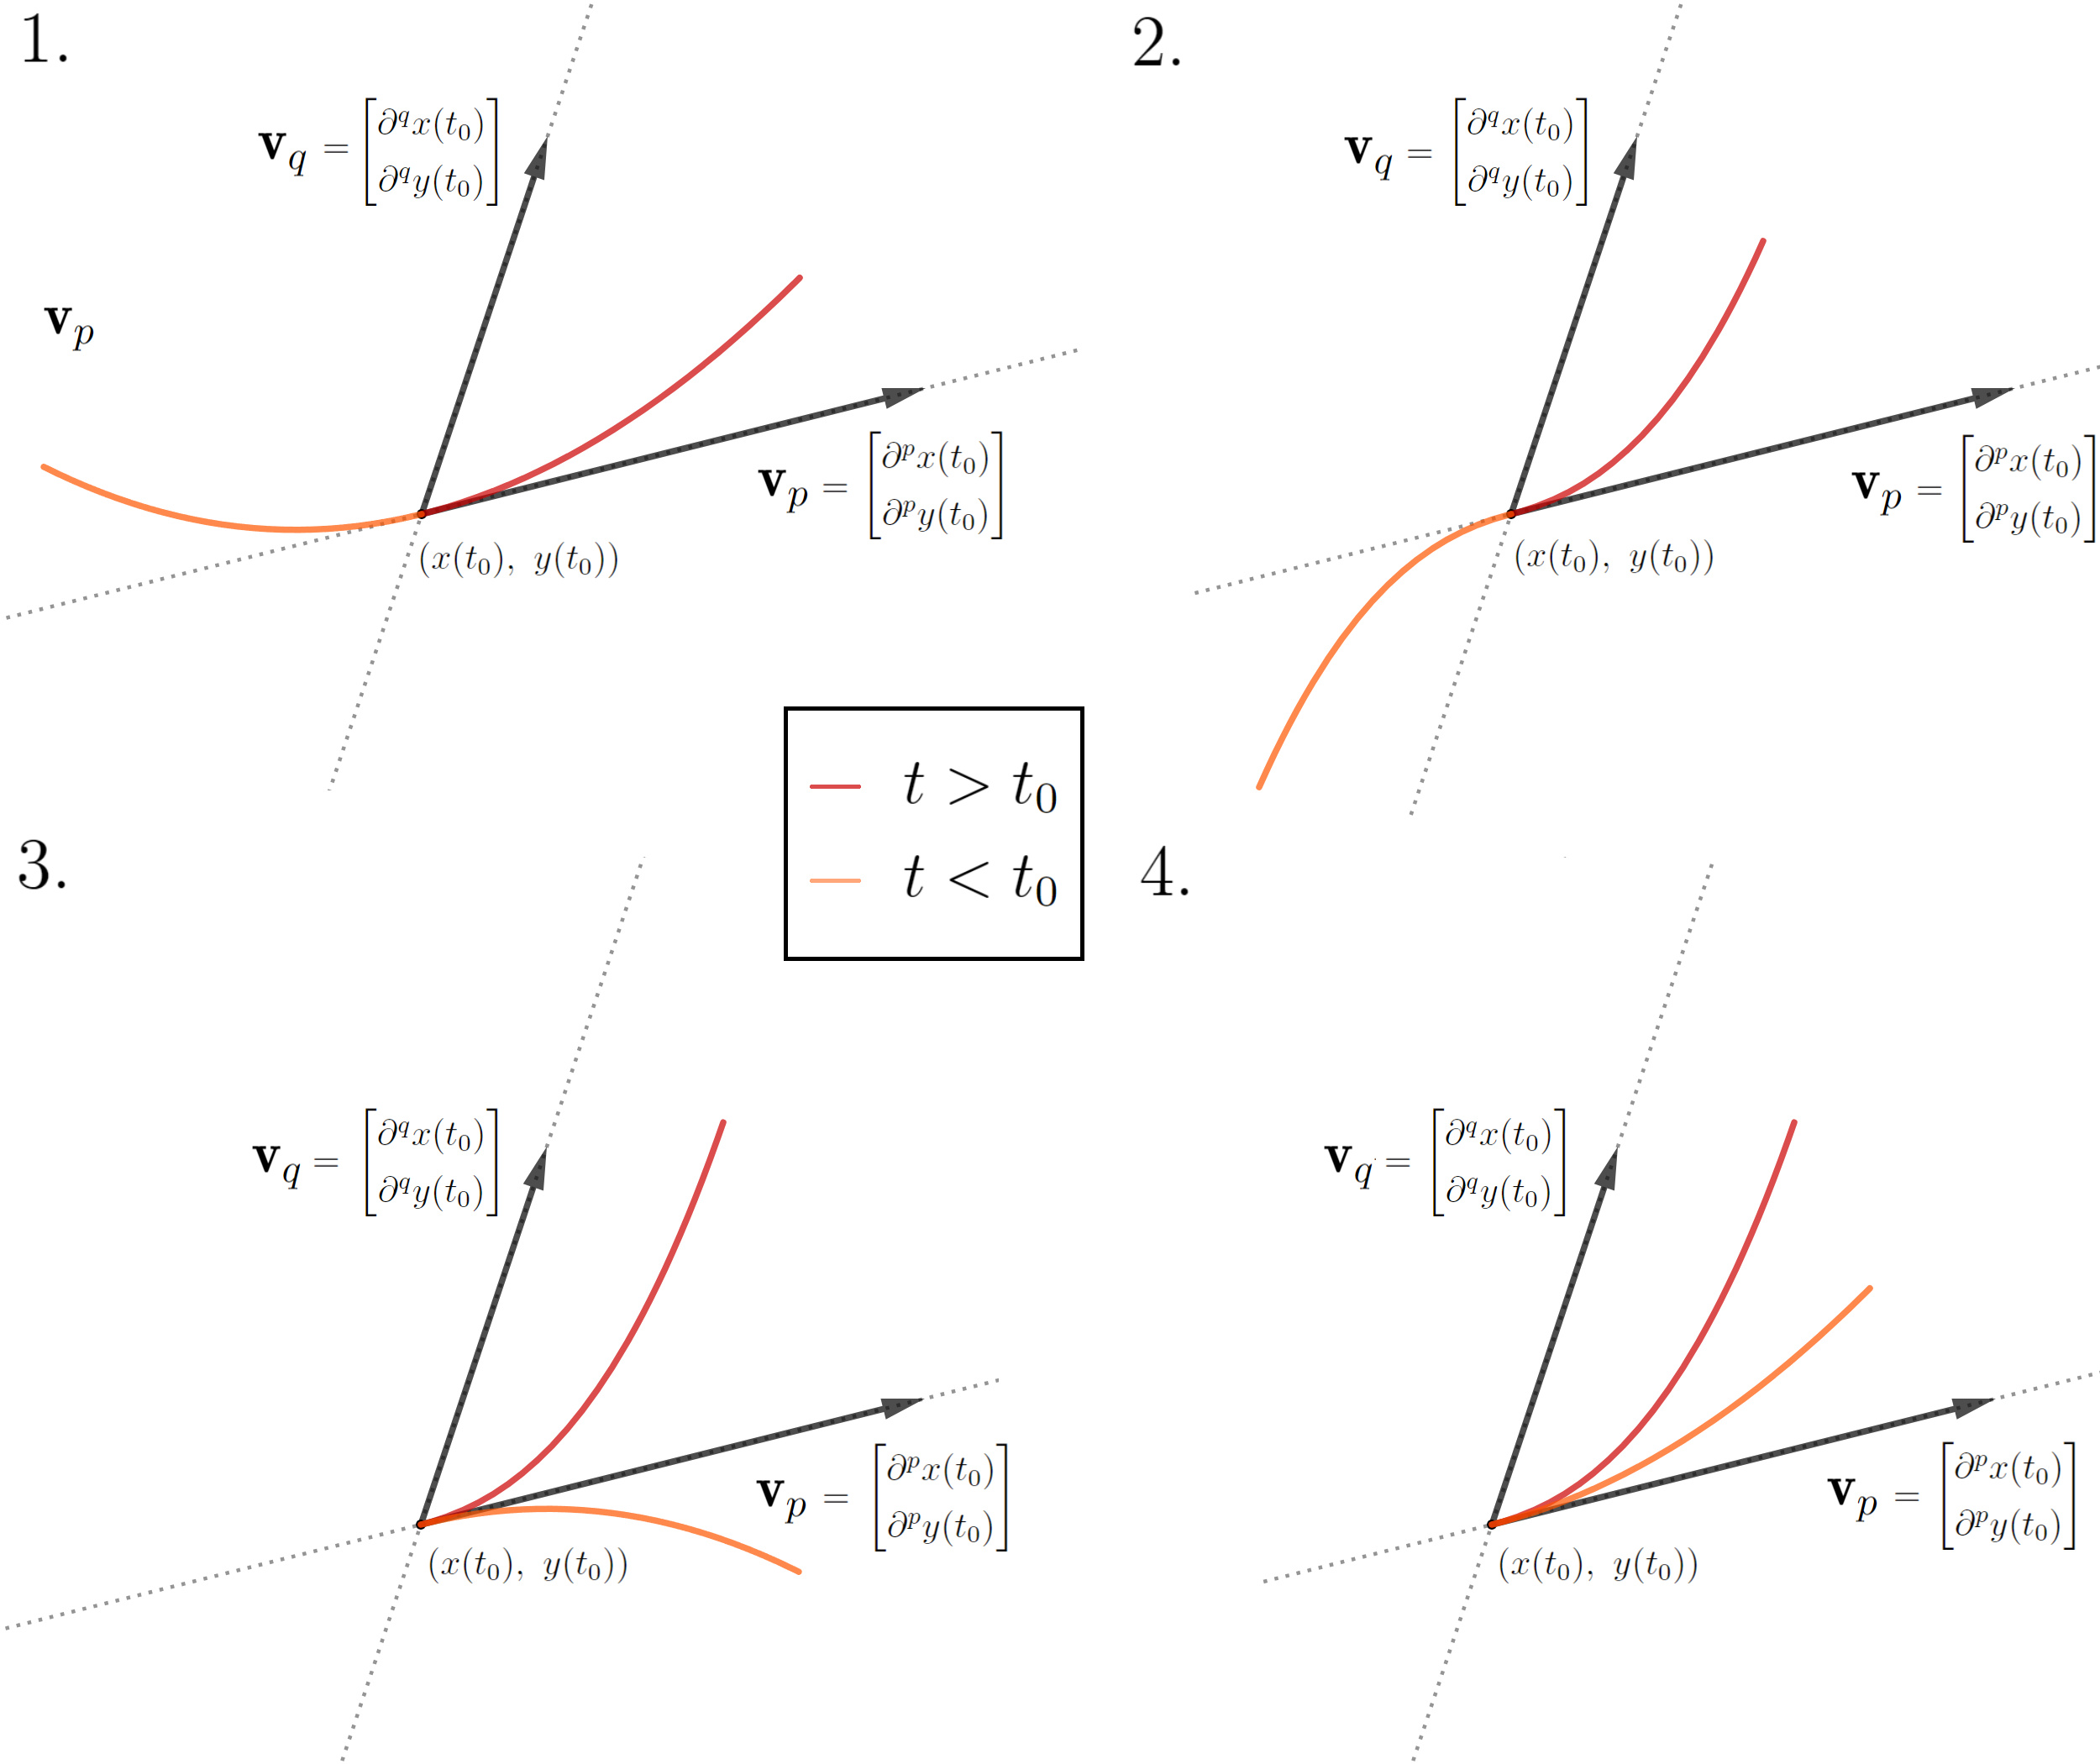
\includegraphics[width=\textwidth]{tu/参数曲线局部展开1.png}
    \caption*{\texttt{参变曲线的局部性质:根据$p,q$奇偶性分为四类情况}}
\end{figure}

参变映射在一点有定义时,可以按以上方法分析。此外,也有参变映射在一点附近有定义,但在该点无定义的情况。
比如$x(t)$或$y(t)$在$t$趋于$t_0$时趋于无穷,或者两者皆然。我们把这种局部情况称为参变曲线\textbf{局部的渐近行为}。

举例来说,考虑参变曲线
\begin{align*}
    f: (0; +\infty) &\rightarrow \mathbb{R}^2 \\
    t\quad &\mapsto\left\{
        \begin{array}[]{rl}
            x(t) &\displaystyle = \frac{1}{t} \\
            y(t) &= t^2\\
        \end{array}
    \right.
\end{align*}
曲线在$t=0$处无定义,但我们需要研究曲线在$t=0$附近的样子。$t>0$趋于$0$时,$x(t)$趋于正无穷,而$y(t)$趋于$0$。
因此,曲线逐渐趋于直线$y = 0$,我们说$y = 0$是曲线在$t=0$处的\textbf{水平渐近线}。

一般来说,如果$t$趋于$t_0$时,$x(t)$趋于正(负)无穷,而$y(t)$趋于某实数$y_0$,那么$y = y_0$是曲线在$t_0$处的水平渐近线。
如果$t$趋于$t_0$时,$y(t)$趋于正(负)无穷,而$x(t)$趋于某实数$x_0$,那么$x = x_0$是曲线在$t_0$处的\textbf{竖直渐近线}。
总之,曲线在局部的渐近行为,表现为无限靠拢渐近线,而具体方向则取决于无穷的正负号。
要注意的是,$t$从$t_0$两侧收敛到$t_0$时,渐近行为要分开讨论。

如果$t$趋于$t_0$时,$x(t)$、$y(t)$都趋于无穷,那么我们需要对这两个无穷大进行比较。
\begin{itemize}
    \item 如果$x(t)$是$y(t)$的高阶无穷大,那么曲线趋于竖直,类似曲线$y = x^2$在$x$趋于无穷时的情况。我们称曲线在$t_0$处\textbf{渐近竖直}。
    \item 如果$y(t)$是$x(t)$的高阶无穷大,那么曲线趋于水平,类似曲线$y^2 = x$在$x$趋于无穷时的情况。我们称曲线在$t_0$处\textbf{渐近水平}。
    \item 如果$\frac{y(t)}{x(t)}$在$t_0$处有极限$a$,那么曲线的渐近行为类似于直线$y = ax$。我们称曲线在$t_0$处\textbf{渐近方向}为向量$(1,\,\,a)$\footnote{或$(-1,\,\,-a)$,取决于$x$、$y$趋于无穷的正负号。下同。}。
    \item 如果曲线有渐近方向$(1, \,\,a)$,则研究$y(t) - ax(t)$。如果它在$t_0$处有极限$b$,那么$y = ax + b$为曲线在$t=0$处的渐近线。如果$y(t) - ax(t)$趋于无穷,那么曲线的渐近行为类似于倾斜的抛物线,我们说曲线在$t_0$处\textbf{抛物渐近}$y = ax$。
\end{itemize}

\begin{et}
    \mbox{} \\
    研究参变曲线:% 例题
    \begin{align*}
        f: (-\infty;0) &\rightarrow \mathbb{R}^2 \\
        t\quad &\mapsto\left\{
            \begin{array}[]{rl}
                x(t) &=2t + t^2 \\
                y(t) &\displaystyle = 2t - \frac{1}{t^2}\\
            \end{array}
        \right.
    \end{align*}
    在$t=-1$附近的性质。
\end{et}

\begin{so}
    参变映射在$t=-1$处的值为$(-1, \,\,-3)$,函数$x$、$y$在该处连续且可微。
    $$
    \left\{
        \begin{array}[]{rl}
            \partial x(t) &=2 + 2t \\
            \partial y(t) &\displaystyle = 2 + \frac{2}{t^3}\\
        \end{array}
    \right.
    $$
    所以
    $$
    \left\{
        \begin{array}[]{rl}
            \partial x(-1) &= 0 \\
            \partial y(-1) & 0\\
        \end{array}
    \right.
    $$
    零向量无法作为切向量,因此继续求二次微变:
    $$
    \left\{
        \begin{array}[]{rl}
            \partial^2 x(t) &=2 \\
            \partial^2 y(t) &\displaystyle = - \frac{6}{t^4}\\
        \end{array}
    \right.
    $$
    因此在$t=-1$处,二次微变向量$\mathbf{v}_2 = (2, \,\,-6)$,可以作为切向量,$p=2$。

    继续考察高次微变。计算可知$t=-1$处的三次微变向量$\mathbf{v}_3 = (0, \,\,-24)$,与$\mathbf{v}_2$不共线。
    于是$q=3$。
    
    我们得到切向量为$(1,\,\,-3)$,次方向向量为$(0,\,\,-1)$。$p=2$为偶数,$q=3$为奇数。
    这说明曲线在$t=-1$处有顺折点。
\end{so}

\begin{figure}[h] 
    % \vspace{-4pt}
    \centering
    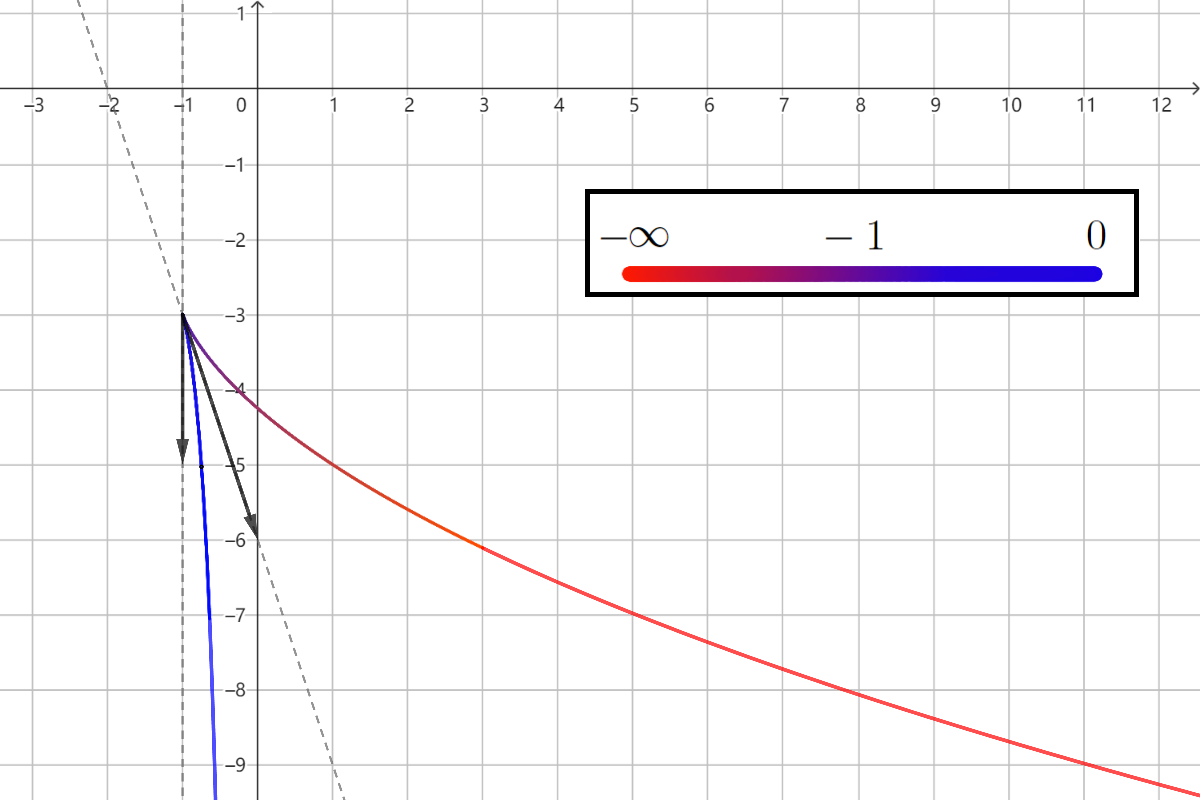
\includegraphics[width=0.8\textwidth]{tu/曲线局部渐近行为01.png}
    \caption*{\texttt{$t$经过$-1$时,曲线在$(-1, \,\,-3)$处停驻并顺折}}
\end{figure}

\begin{et}
    \mbox{} \\
    研究参变曲线:% 例题
    \begin{align*}
        f: (0;+\infty) &\rightarrow \mathbb{R}^2 \\
        t\quad &\mapsto\left\{
            \begin{array}[]{rl}
                x(t) &\displaystyle = t^2 + \frac{2}{t} \\
                y(t) &\displaystyle = t + 3 + \frac{1}{t}\\
            \end{array}
        \right.
    \end{align*}
    在$t=0$附近的性质。
\end{et}

\begin{so}
    当$t$趋于$0^+$时\footnote{指$t>0$且趋于$0$。下同。},$x(t)$和$y(t)$都趋于正无穷。研究两者之比:
    \begin{align*}
        \frac{y(t)}{x(t)} = \frac{t + 3 + \frac{1}{t}}{t^2 + \frac{2}{t}} = \frac{t^2 + 3t + 1}{t^3 + 2}.
    \end{align*}
    因此 
    $$ \lian{t\to 0^+} \frac{y(t)}{x(t)} = \lian{t\to 0^+} \frac{t^2 + 3t + 1}{t^3 + 2} = \frac{1}{2}. $$
    这说明渐近方向为$(2,\,\,1)$。继续研究$y(t) - \frac{1}{2}x(t)$。
    \begin{align*}
        y(t) - \frac{1}{2}x(t) &= t + 3 + \frac{1}{t} - \frac{1}{2}\left(t^2 + \frac{2}{t}\right) \\
        &= t + 3 - \frac{t^2}{2}.
    \end{align*}
    因此
    $$ \lian{t\to 0^+} y(t) - \frac{1}{2}x(t) = \lian{t\to 0^+} t + 3 - \frac{t^2}{2} = 3. $$
    这说明$t$趋于$0^+$时,曲线有渐近线:$y = \frac{1}{2}x + 3$。

    $y(t) - \frac{1}{2}x(t) - 3 = t + \olim{t}$,因此,当$t>0$足够接近$0$的时候,曲线在渐近线上方,与渐近线的距离趋于$0$。
\end{so}

\begin{figure}[h] 
    % \vspace{-4pt}
    \centering
    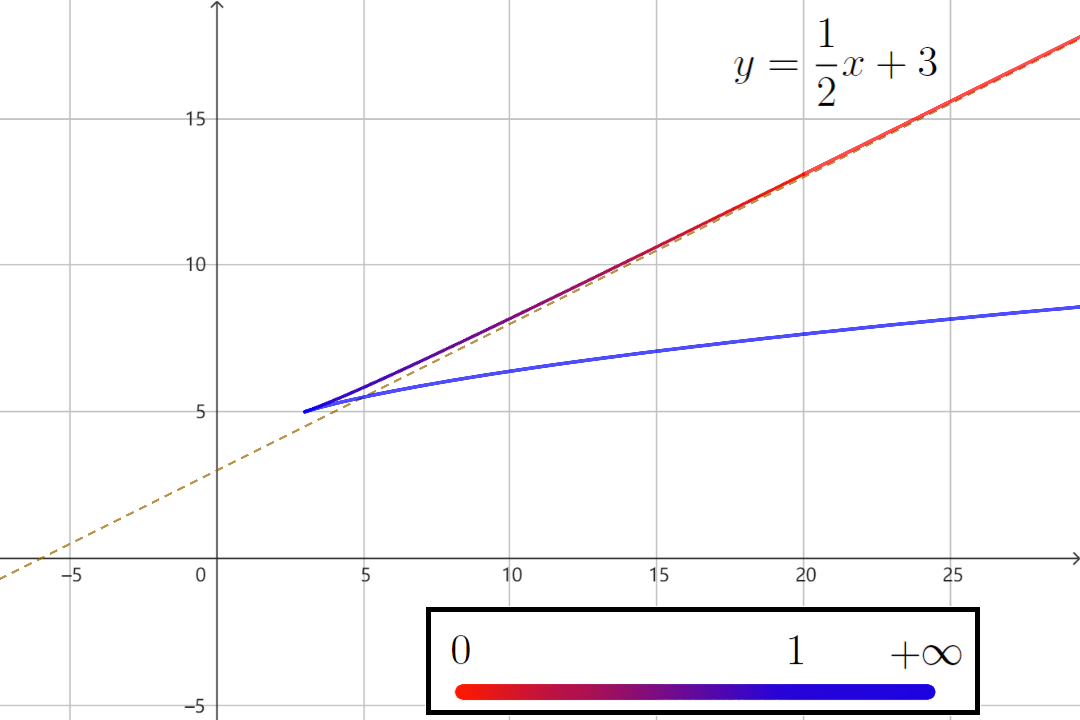
\includegraphics[width=0.8\textwidth]{tu/曲线局部渐近行为02.png}
    \caption*{\texttt{$t$趋于$0^+$时({\color{red}红}),曲线趋于渐近线}}
\end{figure}

\begin{sk}
    \mbox{} \\
    \indent 1. 为什么参变曲线有切向量为零向量的情况,而函数曲线没有这样的情况?\\
    \indent 2. 如果参变量趋于无穷时,参变映射$x$、$y$趋于定值$x_0$、$y_0$,如何研究曲线在$(x_0,\,\,y_0)$附近的性质?\\
    \indent 3. 如果参变量趋于$t_0$时,参变映射$x$或$y$趋于无穷,$x$、$y$的正负号如何影响曲线在局部的渐近行为?分情况讨论。\\
    \indent 4. 能否用关于极坐标的参变映射表示平面曲线?如何研究相关的局部性质?
\end{sk}

\begin{xt}
    \mbox{} \\
    \indent 1. 研究以下参变曲线在$t=0$附近的性质:
    \begin{align*}
        1).\quad f: \mathbb{R} &\rightarrow \mathbb{R}^2 & \quad 2).\quad f: \mathbb{R} &\rightarrow \mathbb{R}^2 \\
        t\quad &\mapsto\left\{
            \begin{array}[]{rl}
                x(t) &= t + 2t^2 - t^3 \\
                y(t) &= t + 2t^2 - t^7 \\
            \end{array}
        \right.
        & \quad 
        t\quad &\mapsto\left\{
            \begin{array}[]{rl}
                x(t) &= t^2 - t \\
                y(t) &= t^2 + t^3 \\
            \end{array}
        \right.
    \end{align*}
    \begin{align*}
        \;\;3).\quad f: \mathbb{R} &\rightarrow \mathbb{R}^2 &  4).\quad f: \mathbb{R} &\rightarrow \mathbb{R}^2 \\
        \;\;t\quad &\mapsto\left\{
            \begin{array}[]{rl}
                x(t) &= t^2 + 3t^3 + t^4 \\
                y(t) &= t^4 - 2t^2 - 6t^3 \\
            \end{array}
        \right.
        & 
        t\quad &\mapsto\left\{
            \begin{array}[]{rl}
                x(t) &= t^2 + 2t^3 \\
                y(t) &= t^3 + t^5 \\
            \end{array}
        \right.
    \end{align*}
    \indent 2. 考虑参变曲线:
    \begin{align*}
        f: [0;+\infty) &\rightarrow \mathbb{R}^2 \\
        t\quad &\mapsto\left\{
            \begin{array}[]{rl}
                x(t) &\displaystyle = \frac{t}{1 + t^4} \\
                y(t) &\displaystyle = \frac{t^3}{1 + t^4} \\
            \end{array}
        \right.
    \end{align*}
    \indent 2.1. 比较$f(t)$和$\displaystyle f\left(\frac{1}{t}\right)$,能得到什么结论?这说明曲线具有什么性质?证明:可以将曲线研究范围缩减到$[0;1]$。\\
    \indent 2.2. 研究$x(t)$和$y(t)$在$[0;1]$上的性质,据此画出曲线的形状。\\
    \indent 3. 考虑参变曲线:
    \begin{align*}
        f: \mathbb{R} &\rightarrow \mathbb{R}^2 \\
        t\quad &\mapsto\left\{
            \begin{array}[]{rl}
                x(t) & = 2\cos{t} - \cos{2t} \\
                y(t) & = 2\sin{t}\, - \sin{2t} \\
            \end{array}
        \right.
    \end{align*}
    \indent 3.1. 证明:随着$t$在$\mathbb{R}$中变化,$f$周期性沿着闭曲线运动。找出最小的周期$T$。\\
    \indent 3.2. 证明:$f$的轨迹关于$x$轴对称。因此,可以将曲线研究范围缩短。给出合适的研究区间。\\
    \indent 3.3. 研究$x(t)$和$y(t)$在该区间上的性质,据此画出曲线的形状。\\
    \indent 4. 研究以下参变曲线在$t=0$附近的性质:
    \begin{align*}
        1).\quad f: \mathbb{R}_{\geqslant 0} &\rightarrow \mathbb{R}^2 & \quad 2).\quad f: \mathbb{R}_{\geqslant 0} &\rightarrow \mathbb{R}^2 \\
        t\quad &\mapsto\left\{
            \begin{array}[]{rl}
                x(t) &\displaystyle = \frac{1+t^2}{t} \\
                y(t) &\displaystyle = 2 - \frac{1}{t} \\
            \end{array}
        \right.
        & \quad 
        t\quad &\mapsto\left\{
            \begin{array}[]{rl}
                x(t) &\displaystyle = \frac{1+t}{t^2} \\
                y(t) &\displaystyle = \frac{1-2t}{t^2} \\
            \end{array}
        \right.
    \end{align*}
    \begin{align*}
        \;\;3).\quad f: \mathbb{R}_{\geqslant 0} &\rightarrow \mathbb{R}^2 &  4).\quad f: \mathbb{R}_{\geqslant 0} &\rightarrow \mathbb{R}^2 \\
        \;\;t\quad &\mapsto\left\{
            \begin{array}[]{rl}
                x(t) &\displaystyle = \frac{1+t}{t^2} \\
                y(t) &\displaystyle = 2 - \frac{1}{t} \\
            \end{array}
        \right.
        & 
        t\quad &\mapsto\left\{
            \begin{array}[]{rl}
                x(t) &\displaystyle = 1 - \frac{1+t}{t^2} \\
                y(t) &\displaystyle = 2 - \frac{1}{t^2} \\
            \end{array}
        \right.
    \end{align*}
    \indent 5. 考虑参变曲线:
    \begin{align*}
        f: \mathbb{R}^* &\rightarrow \mathbb{R}^2 \\
        t\quad &\mapsto\left\{
            \begin{array}[]{rl}
                x(t) &\displaystyle = t + \frac{1}{t} \\
                y(t) &\displaystyle = t + \frac{1}{2t^2} \\
            \end{array}
        \right.
    \end{align*}
    \indent 5.1. 考虑$t$趋于正负无穷时$x(t)$和$y(t)$的变化,说明曲线此时的性质。\\
    \indent 5.2. 考虑$t$趋于$0^+$时$x(t)$和$y(t)$的变化,说明曲线此时的性质。\\
    \indent 5.3. 考虑$t$趋于$0^-$时$x(t)$和$y(t)$的变化,说明曲线此时的性质。\\
    \indent 5.4. 说明$t$趋于$-1$时曲线的局部性质。\\
    \indent 5.5. 说明$t$趋于$1$时曲线的局部性质。\\
    \indent 5.6. 研究$x(t)$和$y(t)$的变化,画出曲线的形状。
\end{xt}


\chapter{广义积合}

\section{一般区间上的积合}

我们已经讨论过闭区间$[a;b]$上连续函数的积合。对于一般的区间、一般的函数,是否能定义积合呢?

\begin{ex}
    \mbox{} \\
    \indent 1. 函数$x\mapsto\frac{1}{x}$在$[0;1]$上是否有积合?\\
    \indent 2. 函数$x\mapsto\frac{1}{x^2}$在$[1;+\infty)$上是否有积合?
\end{ex}

\begin{figure}[h] %this figure will be at the right
    \vspace{4pt}
    \centering
    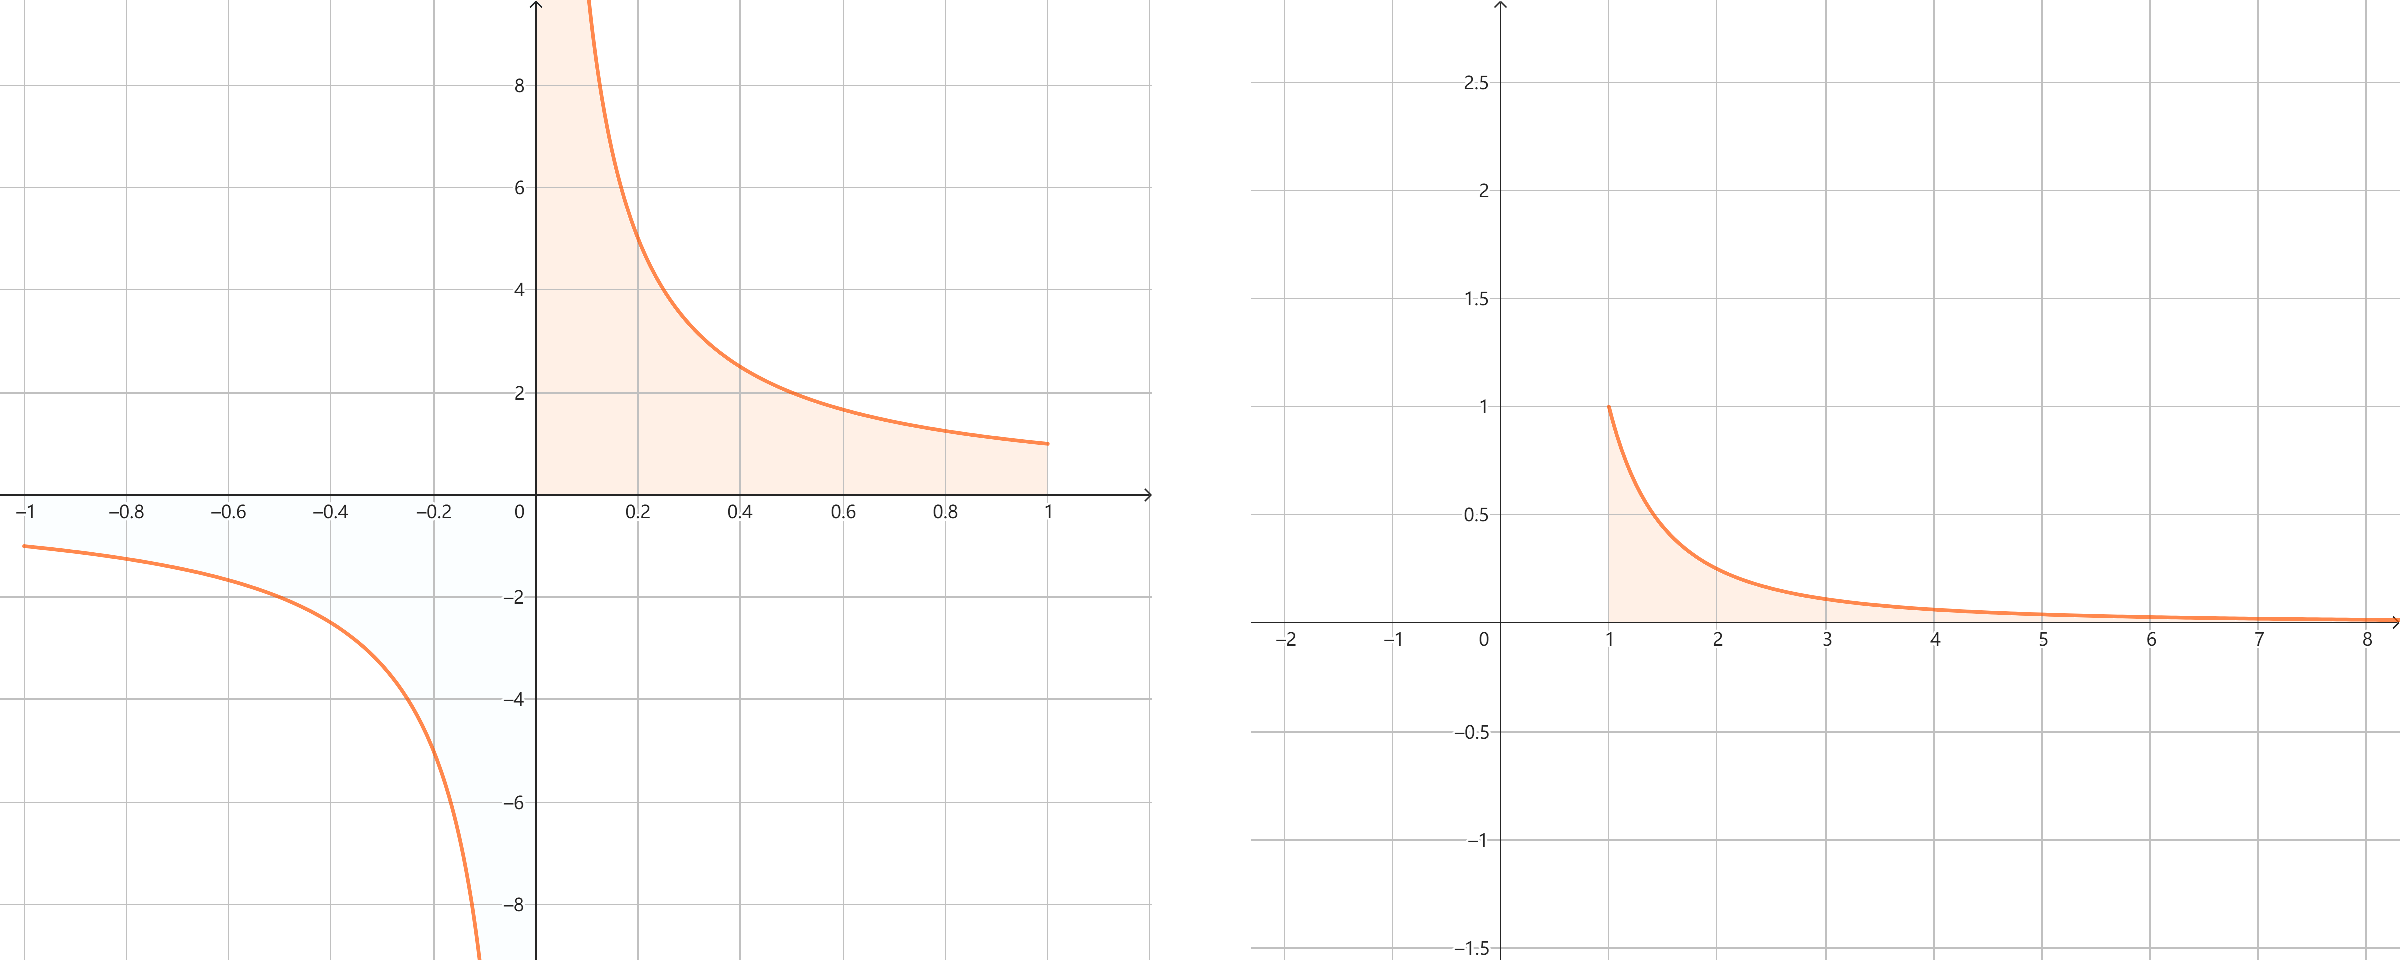
\includegraphics[width=0.9\textwidth]{tu/广义积分1.png}
    \caption*{\texttt{函数}$x\mapsto\frac{1}{x}$(左)、$x\mapsto\frac{1}{x^2}$(右)}
\end{figure}

第一个例子看起来不值得讨论,因为$x\mapsto\frac{1}{x}$甚至不总在$[0;1]$上有定义:$x=0$时,函数无定义。
不过,如果直接看函数的图像,我们能理解这个问题想问什么:如果把积合看作函数与$x$轴之间的图形的面积,那么,
$x\mapsto\frac{1}{x}$这种“无界”的图形是否有面积?

这也是处理一般区间上函数积合时会遇到的问题:闭区间上的连续函数总是有界的,而一般区间上的函数不一定有界。
对于这样的函数,我们能否定义积合呢?

一般来说,以目前的知识,我们无法给任意的函数在任意区间上定义积合。但是,对于一部分“比较好”的函数,我们可以定义积合。

比如,函数$f: x\mapsto\frac{1}{x}$虽然在$[0;1]$上不连续,甚至有未定义的点。但我们可以做一些“修补”。
首先,我们可以给$x=0$处补上定义,比如设$f(0) = 0$。这些工作有助于我们讨论积合的问题,
但不意味着改变函数是否可积的本质。

以上修补过的$f$仍然在$0$处不连续。我们无法直接讨论曲线到$x$轴部分的面积。但我们知道$f$在$(0;1]$上连续。
因此,对任意$a\in(0;1)$,$f$在闭区间$[a;1]$上连续。我们可以求出$f$在$[a;1]$上的面积,然后把$a$趋于$0$。
如果无论$a$以什么方式趋于$0$,面积都趋于一个极限,就定义这个极限为$f$在$[0;1]$上的面积。

首先求$f$在$[a;1]$上的积合:
$$ \int_a^1 f = \ln{1} - \ln{a} = -\ln{a}. $$
这说明$f$在$[a;1]$上的面积是$-\ln{a}$。而$a$趋于$0$时,$-\ln{a}$趋于正无穷。这说明$f$在$[0;1]$上的“面积”是无穷大,
我们说$f$在$[0;1]$上不可积。

第二个例子则比较好理解,因为$f:x\mapsto \frac{1}{x^2}$在$[1;+\infty)$上有定义。我们同样尝试用极限的方式定义函数曲线到$x$轴
的面积。首先求$f$在$[1;a]$上的积合,其中$a>1$:
$$ \int_1^a f = -\frac{1}{a} - (-1) = 1 - \frac{1}{a}. $$
因此$a$趋于正无穷时,$f$在$[1;a]$上的积合趋于$1$。我们说$f$在$[1;+\infty)$上可积。

这样,我们就把积合扩展到定义在一般区间上的连续函数。我们称这种积合为\textbf{广义积合}\footnote{不至于混淆时,也可以简称为积合。}:
\begin{df}
    设函数$f$在半开区间$[a;b)$上连续\footnote{$b$可以是无穷。}。如果当$x$趋于$b$时,$f$在$[a;x]$上的积合总趋于某个极限,
    就说这个极限是$f$在$[a;b)$上的积合,即:
    $$ \int_a^b f = \lian{x\to b^-} \int_a^x f. $$
\end{df}

定义中我们只讨论了区间一端的问题。不过,对于开区间$(a;b)$,我们显然可以先将它截为两段:$(a;c]$、$[c;b)$(其中$c$为区间内任意一点),
然后分别研究这两段是否可积。如果在$(a;c]$、$[c;b)$上都可积,就定义$f$在$(a;b)$上的积合为两段上积合的和。
$$ \int_a^b f = \lian{x\to a^+} \int_x^c f + \lian{x\to b^-} \int_c^x f. $$ 

第一个例子中,我们还“修补”了另一个问题,就是函数在特定点的值的问题。直观来看,函数在单一点是否有定义,或者取不同的值,
不应该改变函数在整个区间上的积合。因为积合是曲线到$x$轴的面积,是一个整体性质。

为此,我们引入分段连续函数的定义:
\begin{df}{\textbf{分段连续函数}}
    设函数$f$在区间$I$上有定义。如果能找到$I$的分割$x_0, x_1, \cdots, x_n$\footnote{其中$x_0$、$x_n$可以是无穷。},
    使得$f$在各个子区间$(x_i;x_{i+1})$上都连续,就说$f$在$I$上(关于该分割)\textbf{分段连续}。
\end{df}
显然,连续函数不论如何分割,总是分段连续的。但也有函数只分段连续而不在整个区间上连续。
比如我们见过的阶梯函数,就是分段连续的不连续函数。

对于分段连续函数,我们可以通过逐段检查,确定它是否可积,并且求出积合。

容易验证广义积合仍然满足积合的基本性质:
\begin{enumerate}
    \item 如果$f$在$I$上可积,且$f$在有限个点以外都大于等于$0$,则其积合大于等于$0$。
    \item 设$a$、$b$、$c$是数轴上的三点,则$\int_a^b f + \int_b^c f = \int_a^c f$。
    \item 设$f$、$g$在$I$上可积,$a, b$为系数,则$ a \int_I f + b \int_I g = \int_I (af + bg) $。
    \item 函数$x\mapsto f\left(\frac{x}{c}\right)$在$[ac; bc]$上的积合,等于$c\int_a^b f$。
    \item 函数$x\mapsto f(x-c)$在$[a+c;b+c]$上的积合,等于$\int_a^b f$。
    \item 如果$f$在区间上的值总介于$m$、$M$之间,那么$m(b - a) \leqslant \int_a^b f \leqslant M(b - a)$。
\end{enumerate}

如果$f$在$I$上有界,那么它在$I$上的广义积合就是它在$I$上的积合。

广义积合与微变也有互逆的关系。比如说,如果$f$在$(a;b]$上可微,且在$a$有右极限,那么:
$$ \int_a^b \partial f = f(b) - \lian{x\to a^+} f.$$
类似地,如果$f$在$[a;b)$上可微,且在$b$有左极限,那么:
$$ \int_a^b \partial f = \lian{x\to b^-} f - f(a).$$

\begin{sk}
    \mbox{} \\
    \indent 1. 假设函数在一点$a$附近(不包括$a$)连续,但在$a$处不连续。这时,不连续的情况可以分成哪几种?其中哪些可以“修补”成连续函数?\\
    \indent 2. 为什么说函数在有限个点上的取值不影响它在区间上的积合?函数在无限个点上的取值是否影响呢?给定区间$I$的子集$D$,
    你认为当$D$满足什么条件的时候,$f$在$D$上的取值会影响它在区间上的积合?\\
    \indent 3. 小明认为,$x\mapsto\frac{1}{x}$在$(0;1]$上的面积是正无穷,在$[-1;0)$上面积是负无穷,所以在$[-1;1]$上面积为$0$。你怎么看?
\end{sk}

\begin{xt}
    \indent 1. 计算以下积合。$a$趋于给定值时,积合是否收敛?\\    
    \begin{align*}
        1).& \int_a^{1} \frac{\ln{x}}{x} , \; a\to 0^+  &2).& \int_1^{a} e^{-x},  \; a\to +\infty \\[3pt]
        3).& \int_0^{a} \frac{1}{\sqrt{1 - x^2}}, \; a\to 1^-   & 4).& \int_a^{1} \sin{\frac{1}{x}}, \; a\to 0^+ 
    \end{align*}
    \indent 2. 计算以下广义积合。\\    
    \begin{align*}
        1).& \int_0^{+\infty} \frac{1}{x\ln^2{x}} ,  &2).& \int_0^{+\infty} xe^{-x^2} \\[3pt]
        3).& \int_0^{+\infty} \frac{1}{(1 + e^{x})^2},  & 4).& \int_0^{+\infty} \frac{e^{-\sqrt{x}}}{\sqrt{x}}
    \end{align*}
    \indent 3. 仿照极限的定义,具体写出“连续函数在$[1;+\infty)$上可积”的定义。\\

\end{xt}

%%% 
\section{广义可积函数}

下面来看一些经典函数的广义积合。

首先来看函数在某点附近不连续导致的广义积合。

考虑函数$x\mapsto x^{-a}$,其中$a>0$为系数。它在$0$处无定义,在$0$右侧趋于正无穷。它是否在$(0;1]$上可积?

对$t>0$,计算它在$[t;1]$上的积合。$a=1$时,我们知道函数不可积。$a\neq 1$时,
\begin{align*}
    \int_t^1 x^{-a} = \frac{1^{1-a}}{1 - a} - \frac{t^{1-a}}{1 - a} = \frac{1 - t^{1-a}}{1-a} 
\end{align*}

$a<1$时,随着$t$趋于$0$,$t^{1-a}$趋于$0$,因此函数在$(0;1]$上可积,积分为$\frac{1}{1-a}$。

$a>1$时,随着$t$趋于$0$,$t^{1-a}$趋于无穷,因此函数在$(0;1]$上不可积。

考虑函数$x\mapsto \ln{x}$,它在$0$处无定义,在$0$右侧趋于正无穷。它是否在$(0;1]$上有积合?

对$t>0$,计算它在$[t;1]$上的积合。
\begin{align*}
    \int_t^1 \ln{x} = 1\cdot \ln{1} - 1 - (t\cdot\ln{t} - t)= t - t\ln{t} - 1
\end{align*}

$t$趋于$0$时,$t\ln{t}$趋于$0$。因此函数在$(0;1]$上可积,积分为$-1$。

再来看函数在无穷区间上的广义积合。

考虑函数$x\mapsto x^{-a}$,其中$a>0$为系数。它是否在$[1;+\infty)$上可积?

对$t>1$,计算它在$[1;t]$上的积合。

$a=1$时,
\begin{align*}
    \int_1^t x^{-a} = \ln{t} - \ln{1} = \ln{t} 
\end{align*}
$t$趋于无穷时,$\ln{t}$趋于无穷,因此函数在$[1;+\infty)$上不可积。

$a\neq 1$时,它在$[1;t]$上的积合为:
\begin{align*}
    \int_1^t x^{-a} = \frac{t^{1-a}}{1 - a} - \frac{1^{1-a}}{1 - a} = \frac{t^{1-a} - 1}{1-a} 
\end{align*}
$a<1$时,随着$t$趋于无穷,$t^{1-a}$趋于无穷,因此函数在$[1;+\infty)$上不可积。

$a>1$时,随着$t$趋于无穷,$t^{1-a}$趋于$0$,因此函数在$[1;+\infty)$上可积,积分为$\frac{1}{a-1}$。

考虑函数$x\mapsto a^x$,其中$a\in(0;1)$为底数。它是否在$[0;+\infty)$上可积?

对$t>0$,计算它在$[0;t]$上的积合。
\begin{align*}
    \int_0^t a^x = \frac{a^t}{\ln{a}} - \frac{a^0}{\ln{a}} = \frac{a^t - 1}{\ln{a}}
\end{align*}
随着$t$趋于无穷,$a^t$趋于$0$,因此函数在$[0,\infty)$上可积,积分为$-\frac{1}{\ln{a}}$。

\begin{figure}[h] %this figure will be at the right
    \vspace{4pt}
    \centering
    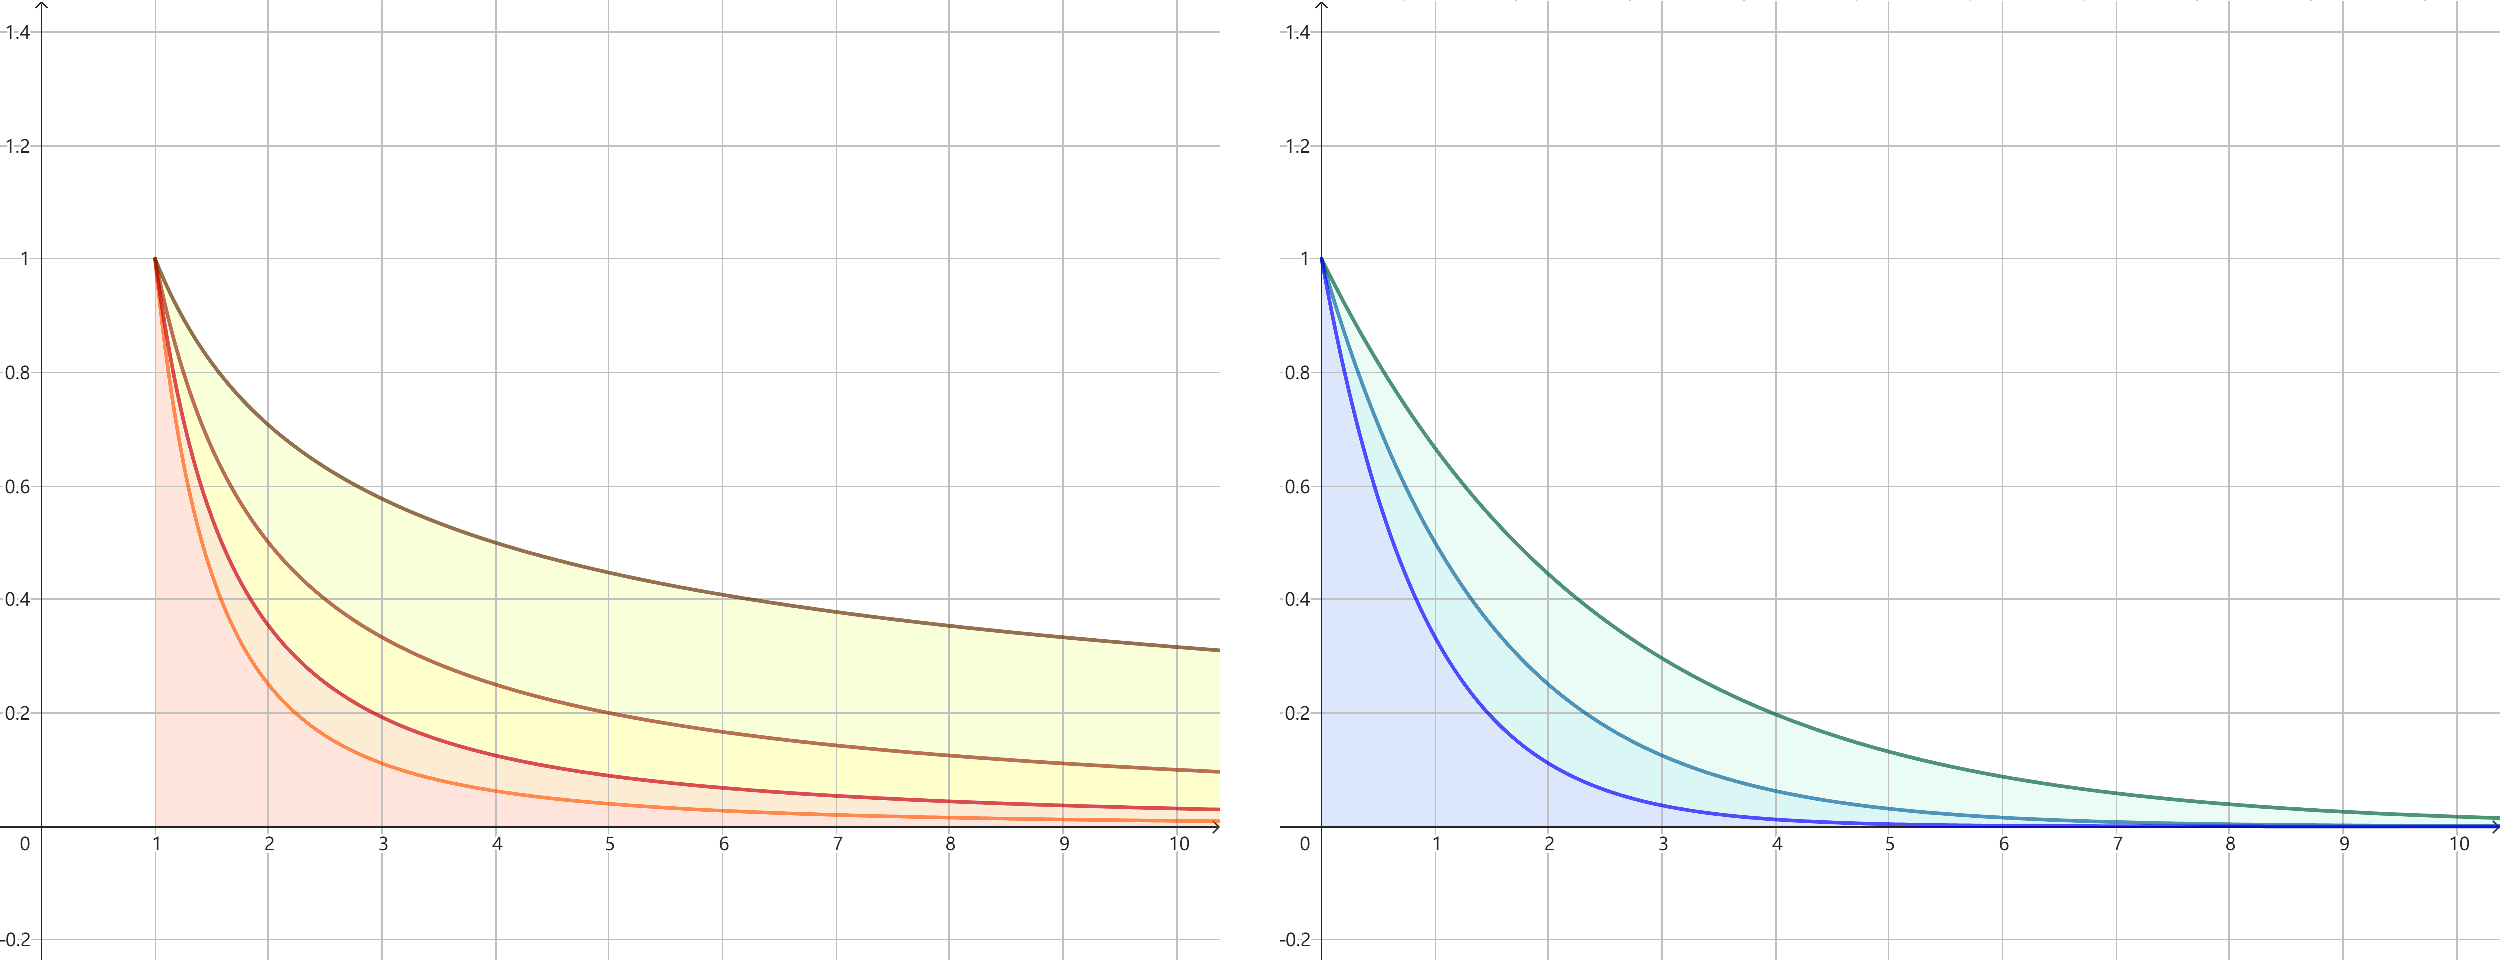
\includegraphics[width=\textwidth]{tu/广义积分2.png}
    \caption*{\texttt{左图:幂函数在}$[1;+\infty)$\texttt{上的面积;右图:指数函数在}$[0;+\infty)$\texttt{上的面积}}
\end{figure}

以上是关于基本的经典函数的讨论,对于更复杂的函数,如何判定它是否广义可积呢?

观察以上的函数在开区间“边缘”的情况,可以发现,造成开区间上面积“无穷”问题的,要么是函数值在开区间端点附近趋于无穷,
要么是开区间为无穷区间——区间长度“无穷”。

我们把前一种情况称为\textbf{无界积合}或\textbf{瑕积合},
把造成问题的端点称\textbf{无界点}或\textbf{瑕点}。而区间为无穷区间的情况,我们称为\textbf{无限积合}。

对于无界积合,直观来说,函数值在瑕点附近急速“爬升”或者“坠落”。
“升”或“落”得越急,曲线到$x$轴的面积就越大;如果“升”或“落”得“太快”,面积就容易变成无穷。

因此,我们可以将函数在无界点附近行为和以上计算过的经典函数进行比较。
如果函数在无界点附近或比可积的经典函数还“慢”,那么可积;如果比不可积的函数还“快”,那么不可积。
而“快慢”程度可以用无穷的阶来具体刻画。

\begin{tm}
    设函数$f$、$g$在区间$I=(a;b]$上分段连续,且在$a$附近同时趋于正无穷。
    \begin{enumerate}
        \item 如果在$a$附近总有$0\leqslant f \leqslant g$,那么只要$g$在$I$上可积,$f$就在$I$上可积。
        \item 如果在$a$附近总有$0\leqslant g \leqslant f$,那么只要$g$在$I$上不可积,$f$就在$I$上不可积。
        \item 如果$f \oveq{a} \Olim{g}$,那么只要$g$在$I$上可积,$f$就在$I$上可积。
        \item 如果$g \oveq{a} \Olim{f}$,那么只要$g$在$I$上不可积,$f$就在$I$上不可积。
        \item 如果$f \oveq{a} \Tlim{g}$,那么$f$在$I$上可积,当且仅当$g$在$I$上可积。
    \end{enumerate}
\end{tm}

举例来说,考虑$(0;1]$上的分段连续函数$f$。如果$f$在$0$点右侧趋于正无穷,那么我们可以将$f$和$x\mapsto x^{-p}$比较。
如果有$p<1$和$r>0$使得$0<x<r$时$f$总受制于$x^{-p}$:
$$ \forall 0<x<r ,\,\,\,\frac{f(x)}{x^{-p}} < M,$$
其中$M$是比值的上界,那么由于$x\mapsto x^{-p}$在$(0;1]$上可积,$f$也在$(0;1]$上可积。

反之,如果$x\mapsto x^{-1}$在$0$右侧附近受制于$f$:
$$ \forall 0<x<r ,\,\,\,\frac{f(x)}{x^{-1}} > M,$$
那么由于$x\mapsto x^{-1}$在$(0;1]$上不可积,$f$也在$(0;1]$上不可积。

再来看无穷积合的情况。
对于无限积合,在无穷远处,如果函数不收敛到$0$,而是收敛到非$0$的数或者趋于无穷,那么显然不可积。
如果函数在无穷远处收敛到$0$,是否就可积呢?

如果函数值(在自变量$x$足够大时)总是正数(或者$0$),那么我们有类似的结论:
\begin{tm}
    设函数$f$、$g$在区间$I=[a;+\infty)$上分段连续。
    \begin{enumerate}
        \item 如果总有$0\leqslant f \leqslant g$,那么只要$g$在$I$上可积,$f$就在$I$上可积。
        \item 如果总有$0\leqslant g \leqslant f$,那么只要$g$在$I$上不可积,$f$就在$I$上不可积。
        \item 如果$0\leqslant f \oveq{+\infty} \Olim{g}$,那么只要$g$在$I$上可积,$f$就在$I$上可积。
        \item 如果$0\leqslant g \oveq{+\infty} \Olim{f}$,那么只要$g$在$I$上不可积,$f$就在$I$上不可积。
        \item 如果$0\leqslant f \oveq{+\infty} \Tlim{g}$,那么$f$在$I$上可积,当且仅当$g$在$I$上可积。
    \end{enumerate}
\end{tm}

考虑$[1;+\infty)$上的分段连续函数$f\geqslant 0$。我们可以将$f$和$x\mapsto x^{-p}$比较。
如果有$p>1$和$A>0$使得$x>A$时$f$总受制于$x^{-p}$:
$$ \forall x>A ,\,\,\,\frac{f(x)}{x^{-p}} < M,$$
其中$M$是比值的上界,那么由于$x\mapsto x^{-p}$在$[1;+\infty)$上可积,$f$也在$[1;+\infty)$上可积。

反之,如果$x\mapsto x^{-1}$在$0$右侧附近受制于$f$:
$$ \forall x>A ,\,\,\,\frac{f(x)}{x^{-1}} > M,$$
那么由于$x\mapsto x^{-1}$在$[1;+\infty)$上不可积,$f$也在$[1;+\infty)$上不可积。

以上讨论中我们加上了函数大于等于$0$的条件。如果函数值可正可负时,情况更加复杂。
我们可以把无限积合与可数个数求和——也就是级数——的情况类比。
讨论级数收敛时,我们将级数分为正项级数和一般的级数,并引入了级数的绝对值、绝对收敛和相对收敛的概念。

对于无限积合,我们引入\textbf{绝对可积}的概念。
对于定义在区间$I$上的函数$f$,如果它的绝对值$|f|: x\mapsto |f(x)|$在$I$上可积,就说$f$绝对可积;
否则就说$f$\textbf{相对可积}。

在$I$上绝对可积的函数,一定相对可积,但反之则不一定。

要注意的是,如果函数在无穷远处没有极限,并不能说明它可积或不可积。比如说,我们可以在足够远处给函数加上一些“小尖刺”。
每个“小尖刺”的面积都很小,不影响可积,但“刺尖”的函数值可以很大,甚至趋于无穷。

具体来说,我们制作这样的“尖角函数”:
\begin{align*}
    f: [0;1] &\rightarrow \mathbb{R} \\
x \;&\mapsto \begin{cases}
    2x & 0\leqslant x \leqslant \frac{1}{2} \\
    1 - 2x & \frac{1}{2} < x \leqslant 1
\end{cases} 
\end{align*}
这个函数的图像是平放在$x$轴上的等腰三角形。它的左端和$0$对齐,底和高都是$1$。我们可以将它拉伸放缩为“尖刺”:
\begin{align*}
   [a;a+b] &\rightarrow \mathbb{R} \\
    x \;&\mapsto h\cdot f\left(\frac{x-a}{b}\right)
\end{align*}
这个函数的图像也是$x$轴上的等腰三角形,只不过底边是$x$轴上的线段$[a;a+b]$,底长为$b$,高为$h$。

取一个在$[1;+\infty)$上可积的非负函数,比如$\displaystyle f_0: x\mapsto \frac{1}{x^2}$。在足够远的地方放置这些“尖刺”,得到以下函数:
$$
g: x\mapsto \begin{cases}
    \displaystyle f_0(x) + 2n f\left(n^3(x - n)\right) & \mbox{如果}\; x \in \left[n;n+\frac{1}{n^3}\right],\; n\in\mathbb{Z}^+ \\
    f_0(x) & \mbox{其他的}\;x
\end{cases}
$$
对任意正整数$n$,函数$g$在区间$\left[n;n+\frac{1}{n^3}\right]$上叠加放置了底边为$\frac{1}{n^3}$,高为$2n$的等腰三角形。它的面积为$\frac{1}{n^2}$。

因此,相对于$f_0$,$g$的面积增加不超过$\displaystyle \sum_{n\geqslant 1} \frac{1}{n^2}$。而$\displaystyle \sum_{n\geqslant 1} \frac{1}{n^2}$是收敛的级数,所以函数$g$也是可积乃至绝对可积的。
然而,$g$的函数值在$n+\frac{1}{2n^3}$处可以达到$2n$,因此没有上限,随着$n$的增大而趋于无穷。

从这个例子可以看出,无限积合的判断比无界积合、级数收敛的判断更复杂。这是由实数集的不可数特性和函数的复杂性决定的。

\begin{sk}
    \mbox{} \\
    \indent 1. 总结非负连续函数的无限积合和正项级数的收敛的相似性。\\
    \indent 2. 为什么讨论无界积合时,没有考虑函数值的正负性?\\
    \indent 3. 广义积合可以看作对函数的积合求极限。是否可以先对函数求极限,再求积合?这两种操作是否等价?\\
    \indent 4. 连续函数在无穷远处不收敛到$0$,是否一定不可积?
\end{sk}

\begin{xt}
    \mbox{} \\
    \indent 1. 以下函数是否在$\mathbb{R}^+$上可积?\\    
    \begin{align*}
        1)\;\;& \frac{1}{x\ln^2{x}} ,  &2)\;\;& \frac{e^{-x^2}}{\sqrt{x}}, \\[3pt]
        3)\;\;& \sin{\frac{1}{x}},  & 4)\;\;& \frac{1}{e^x  - 1}.
    \end{align*}
    \indent 2. 以下积合是否存在?\\    
    \begin{align*}
        1)\;\;& \int_2^{+\infty} \frac{1}{\sqrt{x(x - 1)(x - 2)}},  &2)\;\;& \int_0^{\frac{\pi}{2}} \frac{1}{\sin{x}\cos{x}(1 - e^{-x})}, \\[3pt]
        3)\;\;& \int_0^{1} \frac{\ln{x}}{(1 - x^2)^{\frac{3}{2}}} , & 4)\;\;& \int_0^{\pi} \frac{1}{\sqrt{\sin{x}}}.
    \end{align*}
    \indent 3. $f$是$[1;+\infty)$上的分段连续函数。\\
    \indent 3.1. 证明:如果有正实数$a>1$使得$\lian{t\to+\infty} t^a f(t) = 0$,那么$f$在$[1;+\infty)$上绝对可积。\\
    \indent 3.2. 证明:如果有正实数$c$使得$\lian{t\to+\infty} t f(t) \geqslant c$,那么$f$在$[1;+\infty)$上不可积。\\
    \indent 4. $f$是$(0;1]$上的分段连续函数。\\
    \indent 4.1. 证明:如果有正实数$a<1$使得$\lian{t\to 0^+} t^a f(t) = 0$,那么$f$在$(0;1]$上绝对可积。\\
    \indent 4.2. 证明:如果有正实数$c$使得$\lian{t\to 0^+} t f(t) \geqslant c$,那么$f$在$(0;1]$上不可积。\\
    \indent 5. 当$a$取什么值的时候,以下带参数$a$的函数在$\mathbb{R}^+$上可积?\\
    \begin{align*}
        1)\;\;& \frac{\ln{x}}{x^a} ,  &2)\;\;& \frac{e^{-x} - 1}{x^a}, \\[3pt]
        3)\;\;& \frac{x - \sin{x}}{x^a},  & 4)\;\;& \frac{\arctan{x}}{x^a}. 
    \end{align*}
    \indent 6. 设$f$是$\mathbb{R}^+$上的连续可积函数。\\
    \indent 6.1. 设$\{x_n\}$、$\{y_n\}$为两个趋于正无穷的数列。证明:
    $$ \lian{n\to+\infty}\int_{x_n}^{y_n} f = 0. $$
    \indent 6.2. 证明:$e^{-t\sin{t}}$在$\mathbb{R}^+$上不可积。

\end{xt}

\section{积分的应用}

\chapter{后续}

\begin{appendix}

\chapter{度量以外}
% Oleg Viro, [Metric, neighborhoods, topology](https://www.math.stonybrook.edu/~oleg/mat150-fall16/MetricsNbhdsTopology.pdf)

\section{邻域、开集和闭集}

\begin{df}{\textbf{邻域结构}}\label{df:a-0-0}
    给定一个集合$S$,以及映射$L$:对任意$x\in S$,都有确定的集合$L(x)$。如果它们满足以下条件:
    \begin{enumerate}
        \item $\forall x\in S$,$L(x)$是非空集合,其元素是$S$的子集;
        \item $\forall x\in S$,$\forall U \in L(x)$,$x\in U$;
        \item 只要$U\in L(x)$,$U\subseteq V$,那么$V\in L(x)$;
        \item 只要$U, V\in L(x)$,那么$U\cap V \in L(x)$;
        \item $\forall x\in S$,$\forall U\in L(x)$,$\exists V \in L(x)$,使得$\forall y\in V$,$U\in L(y)$。
    \end{enumerate}
    就说它们是$S$上的一个\textbf{邻域结构}。装备了某个邻域结构$L$的集合$S$称为\textbf{邻域空间},对$S$中任意$x$,$L(x)$的元素称为它的\textbf{邻域}。
\end{df}

\begin{df}{\textbf{开闭结构}}\label{df:a-0-1}
    给定一个集合$S$,以及$S$的一些子集构成的集合$\Omega$。如果$\Omega$的元素满足以下条件:
    \begin{enumerate}
        \item $\Omega$的元素的并集,仍然是$\Omega$的元素;
        \item 有限个$\Omega$的元素的并集,仍然是$\Omega$的元素;
        \item 空集$\varnothing$和$S$都是$\Omega$的元素。
    \end{enumerate}
    就说它是$S$上的\textbf{开闭结构}。装备了某种开闭结构$\Omega$的集合$S$称为\textbf{开闭空间}。$S$的元素称为开闭空间的点,$\Omega$中的元素称为空间的\textbf{开集},开集(关于$S$)的补集称为空间的\textbf{闭集}。
\end{df}

可以看到,邻域结构从特定的点出发定义“相邻”,而开闭结构则不关心特定的点。前者是局部的,后者是整体的。

邻域空间和开闭空间都可以用来讨论空间中点的“附近”“包含”等问题。它们之间有什么联系呢?

在邻域空间中,我们这样定义开集:
\begin{df}{\textbf{邻域空间中的开集}}\label{df:a-0-2}
    给定$S$和其上的邻域结构$L$。$S$的子集$U$为开集当且仅当$U$是其任意元素的邻域,即:
    $$ \forall x\in U, \;\; U\in L(x).$$
\end{df}

在开闭空间中,我们这样定义邻域:
\begin{df}{\textbf{开闭空间中的邻域}}\label{df:a-0-3}
    给定$S$和其上的开闭结构$\Omega$,一点$x\in S$的邻域$N$是包含它的开集的母集,即:
    $$ \exists\, U \in \Omega, \;\; \mbox{使得}\; x\in U \subseteq N.  $$
\end{df}
换句话说,开闭空间中,说$N$是$x$的邻域,就是说$N$里有一个包含$x$的开集。按照这个定义,开集本身就是其中任意点的邻域。
这符合邻域空间中对开集的刻画。反之,按照邻域空间的定义,由于开集是其中的点的邻域,所以它的母集也是该点的邻域。
这也符合开闭空间中对邻域的刻画。

\begin{tm}\label{tm:a-0-0}
    开闭空间中的开集是其任何元素的邻域。
\end{tm}

\begin{proof}
    给定$S$和其上的开闭结构$\Omega$。设$U\in \Omega$是开集,那么$\forall x\in U$,$U$是包含$x$的开集$U$的母集,因而是$x$的邻域。
\end{proof}

在这样的相互定义之下,我们可以证明邻域空间和开闭空间是\textbf{互生}的:我们总可以从给定的邻域空间出发,定义开集,然后这样定义的开集满足开闭空间的定义。
反过来,我们总可以从给定的开闭空间出发,定义邻域,然后这样定义的邻域,满足邻域空间的定义。

\begin{tm}
    给定$S$和其上的开闭结构$\Omega$,以上定义的邻域形成邻域结构。
\end{tm}

\begin{proof}
    我们逐一证明邻域结构的条件得到满足。

    条件一:任一点都有邻域。这是因为$S$在$\Omega$中,$S$是开集,从而$S$是包含任意点的开集$S$的母集,即任一点的邻域。

    条件二:任一点属于它的邻域。给定$x$及其邻域$N$,按照定义$N$是包含$x$的开集的母集,因此包含$x$。

    条件三:一点的邻域的母集是它的邻域。给定$x$及其邻域$N$,按照定义$N$是包含$x$的开集$U$的母集,因此$N$的母集仍然是$U$的母集,从而是$x$的邻域。

    条件四:一点的邻域的交集是它的邻域。给定$x$及其邻域$N_1, N_2$,按照定义,他们分别是包含$x$的开集$U_1, U_2$的母集。
    因此$x\in U_1\cap U_2 \subseteq N_1\cap N_2 $。而按照开闭结构的定义,$U_1\cap  U_2$也是开集。
    这说明$N_1\cap N_2$是$x$的邻域。

    条件五:一点的邻域包含邻域作为子集,并且是子集中任何点的邻域。给定$x\in N$,则有开集$U$使得$x\in U \subseteq N$。根据定理\ref{tm:a-0-0},$U$是其中任何元素的邻域,而$\forall y \in U$,都有$y\in U \subseteq N$。因此$U$就是我们要找的子集。
\end{proof}

\begin{tm}
    给定$S$和其上的邻域结构$L$,以上定义的开集形成开闭结构。
\end{tm}

\begin{proof}
    我们逐一证明开闭结构的条件得到满足。

    条件一:开集的并集仍然是开集。设有开集的集合$I$,$I$中元素都是开集。考虑它们的并集:
    $$ U = \bigcup_{K\in I} K. $$
    按定义,$U$是开集,当且仅当$U$是$U$中任意元素的邻域。因此,我们要证明:$U$是其任意元素的邻域。考虑$x\in U$,则$x$是$I$中某个元素:开集$K$的元素:
    $$ \exists \, K \in I, \;\; x \in K.$$
    于是$K$是$x$的邻域,从而$U$作为$K$的母集,也是$x$邻域。这就证明$U$是开集。

    条件二:有限个开集的交集仍然是开集。设$n$是正整数,考虑$n$个开集:$K_1, K_2, \cdots, K_n$的交集:
    $$ J = \bigcap_{1\leqslant i \leqslant n} K_i.$$
    我们要证明:$J$是其任意元素的邻域。考虑$x\in J$,$\forall i\in [1..n]$,$x\in K_i$,因此$K_i$是它的邻域。
    而邻域的交集仍然是邻域,因此$J$是$x$的邻域。这就证明$J$是开集。

    条件三:空集和全集$S$是开集。首先,$S$是$S$中任意点的邻域的母集,因此是任意点的邻域。这说明$S$是开集。
    其次,空集不包含任一点,所以自然是它的任意元素(如果有的话)的邻域。

\end{proof}

我们把以上构造出来的开闭(邻域)空间称为邻域(开闭)空间\textbf{生出}的空间。

这样自然引出一个问题:如果我们从一个开闭空间出发生出邻域空间,再从这个邻域空间出发生出一个开闭空间。前后两个开闭空间一样吗?

\begin{tm}{\textbf{互生定理}}
    \mbox{} \\
    给定集合$S$,
    \begin{enumerate}
        \item $S$上的开闭空间$\Omega$上生出的邻域空间$L$上生出的开闭空间就是$\Omega$。
        \item $S$上的邻域空间$L$上生出的开闭空间$\Omega$上生出的邻域空间就是$L$。
    \end{enumerate}
\end{tm}

\begin{proof}
    首先,给定$S$上的开闭空间$\Omega$,设$L$是它生出的邻域空间,$\Omega'$是$L$生出的开闭空间。下面证明$\Omega = \Omega'$。
    
    设$U\in\Omega$是开集,则根据定理\ref{tm:a-0-0},$U$是其任意元素的邻域。按定义,$U$是$\Omega'$的开集。

    反之,如果$U$是$\Omega'$的开集。这说明$\forall x \in U$,$U$是$L(x)$的邻域。
    而$L$是$\Omega$生出的邻域空间。按定义\ref{df:a-0-3},可以找到$V_x\subseteq U$,$V_x$是$\Omega$的开集。
    考虑全体$V_x$的并集:
    $$V = \bigcup_{x\in U} V_x. $$
    开闭空间的开集的并集总是开集。因此$V$是$\Omega$中的开集。然而$V$就是$U$!一方面,$\forall x\in U$,$x\in V_x \subseteq V$。这说明$U\subseteq V$。
    另一方面,$\forall x\in U$,$V_x\subseteq U$,所以全体$V_x$的并集$V\subseteq U$。$U, V$互含,说明$U = V$,$U$是$\Omega$的开集。

    $\Omega,\Omega'$的开集相同,因此$\Omega = \Omega'$。

    其次,给定$S$上的邻域空间,设$\Omega$是它生出的开闭空间,而$L'$是$\Omega$生出的邻域空间。下面证明$L=L'$。

    给定$x\in S$,我们证明$L(x)$和$L'(x)$是相同的集合。一方面,设$V\in L'(x)$,它是由$\Omega$中的开集定义的邻域,即它含有某个$\Omega$的开集$x\in U$作为子集。
    而开集$U$是由$L$中邻域定义的,是$U$中任意元素在$L$上的邻域,因此也是$x$的邻域。这说明$V$作为$U$的母集,也是$x$在$L$上的邻域:$V\in L(x)$。

    另一方面,设$V\in L(x)$,我们构造这样的集合$U$:
    $$ U = \{q \in S | V \in L(q)\}. $$
    注意到$V$是$x$的邻域,这说明$x\in U$。此外,$U$中任何元素都有$V$作为邻域,所以属于$V$。这说明$U\subseteq V$。
    再者,给定$x\in U$,它有$V$作为邻域,按邻域的定义,可以找到$x$的邻域$W_x$,使得$W_x \subseteq V$,并且$V$是$W_x$中任何元素的邻域。
    但$U$是所有“$V$是它的邻域”的点的集合,这说明$W_x\subseteq U$。换句话说,$\forall x\in U$,我们都能找到$U$的子集作为$x$的邻域,因此$U$作为其母集也是$x$的邻域。
    这就证明了$U$是$\Omega$的开集。而$V$作为$U$的母集,按定义\ref{df:a-0-3},就是$L'(x)$的元素。

    综上,对任意$x$,$L(x)$和$L'(x)$包含相同的元素。这说明$L=L'$。    
\end{proof}

于是,我们统一了邻域空间和开闭空间这两个概念。以后我们将其统一称为\textbf{有邻空间},将对应的结构统称为\textbf{邻则}。
以后我们讨论邻域和开集的时候,就可以自由地相互转换了。邻域空间中提到的开集,是它生出的开闭空间中的开集,它是它任意元素的邻域;
而开闭空间中某点的邻域,是它生出的邻域空间中的邻域,它总有包含该点的开集作为子集。

以上的推导过于抽象。我们用不严谨的直观想象来打个比方。直观上,我们可以想象这样的图景:一点包含在一个开集里,而开集包含在一个邻域里,就像一个荷包蛋一样。
另一方面,开集可以想象成一个球面:大小也许有限,但没有边。

\begin{sk}
    \mbox{} \\
    \indent 1. 是否有既是开集又是闭集的集合?是否有既不是开集又不是闭集的集合?\\
    \indent 2. 在某个邻域结构$L$里,两点$a$、$b$的邻域集合$L(a), L(b)$交集是空集,这说明什么?如果交集不是空集呢?
\end{sk}

\begin{xt}
    \mbox{} \\
    \indent 1. 证明闭集的基本性质:\\
    \indent 1.1. 空集和全集都是闭集。\\
    \indent 1.2. 有限个闭集的并集是闭集。\\
    \indent 1.3. 闭集的交集是闭集。\\
    \indent 2. \\
    \indent 5.
\end{xt}

一般来说,同一个集合上,是否只有唯一的邻域结构或开闭结构?答案显然是否定的。只要是足够大的集合,就可能产生很多邻域结构或开闭结构。
换句话说,我们有不止一种方法指定什么是一点的“附近”。

给定集合$S$上的各种结构中,有一种情形是我们要指出的:对$S$上的两个开闭结构$\Omega_1, \Omega_2$,如果$\Omega_1$是$\Omega_2$的子集,
就说$\Omega_1$比$\Omega_2$更\textbf{粗略},$\Omega_2$比$\Omega_1$更\textbf{精细}。换句话说,比起$\Omega_1$,
我们用$\Omega_2$能给出更多的开集,能更精细地比较点与点之间的关系。

用邻域结构可以更直观地看到这一点。对$S$上的两个邻域结构$L_1, L_2$,如果对$S$中任意元素$x$,总有$L_1(x) \subseteq L_2(x)$,就说$L_1$比$L_2$更\textbf{粗略},$L_2$比$L_1$更\textbf{精细}。
直观来说,使用$L_2$,我们有更多方法描述一点$x$的“附近”。

\section{开闭空间的基底}

\begin{tm}{\textbf{实数集的经典结构}}\label{tm:a-1-0}
    在实数集$\mathbb{R}$上,考虑所有有界开区间的集合$\mathcal{K}$:
    $$ \mathcal{K} = \{ (a;b) \, | \, a, b \in \mathbb{R} \}$$
    则由$\mathcal{K}$中元素的并集构成的集合:
    $$ \Omega(\mathbb{R}) = \left\{\bigcup_{I \in \mathcal{J}} I \, \Bigg| \,\mathcal{J} \subseteq  \mathcal{K} \right\}.$$
    是$\mathbb{R}$上的开闭结构。我们称$\Omega(\mathbb{R})$为实数集$\mathbb{R}$上的\textbf{经典结构},也叫\textbf{经典邻则}。
    以后提到$\mathbb{R}$上的邻域、开集、闭集等概念,我们都默认是这个经典邻则下的概念。
\end{tm}

\begin{proof}
    逐个验证$\Omega(\mathbb{R})$满足开闭结构的三个条件:

    条件一:$\Omega(\mathbb{R})$是由$\mathcal{K}$中元素的并集构成的集合,因此,$\Omega(\mathbb{R})$中元素的并集,仍然在$\Omega(\mathbb{R})$里。

    条件二:给定两个$\Omega(\mathbb{R})$里的元素,设它们分别是$\mathcal{K}$的子集$\mathcal{J}_1, \mathcal{J}_2$中的开区间的并集。
    考虑它们的交集:
    \begin{align*}
        \left(\bigcup_{I \in \mathcal{J}_1} I\right) \cap \left(\bigcup_{I \in \mathcal{J}_2} I\right) &= \bigcup_{I_1 \in \mathcal{J}_1} \bigcup_{I_2 \in \mathcal{J}_2} (I_1 \cap I_2)   
    \end{align*}
    考察等式右边,每个$I_1 \cap I_2$表示两个有界开区间的交集,这样的集合要么是空集,要么是某个有界开区间,因此总在$\mathcal{K}$里。
    这说明所有形如$I_1 \cap I_2$的并集仍然在$\Omega(\mathbb{R})$里。这说明两个$\Omega(\mathbb{R})$里的元素,交集仍然在$\Omega(\mathbb{R})$里。

    对于一般的正整数$n>2$,重复以上步骤$n-2$次,就可以证明$n$个$\Omega(\mathbb{R})$里的元素交集仍然在$\Omega(\mathbb{R})$里。
    这说明有限个$\Omega(\mathbb{R})$的元素的交集仍然是$\Omega(\mathbb{R})$的元素。

    条件三:首先,$\varnothing = \bigcup_{I \in \varnothing} I $,因此空集在$\Omega(\mathbb{R})$中。
    其次,$\mathbb{R}$可以按如下方式分解为开区间的并集:
    $$ \mathbb{R} = \bigcup_{n\in \mathbb{Z}} (n-1;n+1) . $$
    因此全集$\mathbb{R}$在$\Omega(\mathbb{R})$中。

\end{proof}

上面的验证中,可以发现,交集是最难处理的部分。因为交集让集合“变小”了,而“太小”的集合很容易出现“动不了”的情况,就不再是开集了。
比如,考虑开集的序列:
$$ \left\{ \left(-\frac{1}{n};\frac{1}{n}\right)\right\}_{n\in\mathbb{Z}^+}.$$
从序列里拿出有限项,交集仍然是开区间,但所有项的交集是$\{0\}$,是闭区间,也是我们说的“动不了”的集合。

从以上的定义里,我们发现,可以从一个比较容易理解的、比较“小”的集合出发,构造出整个开闭结构。
整个开闭结构可以看作这个集合里元素的并集,或者不严谨地说,是一种“和”。这让我们想到平直空间的情况。

一般情况下,我们可以定义开闭空间的基底:
\begin{df}
    给定集合$S$和$S$的子集构成的集合$\mathcal{B}$,如果$\mathcal{B}$满足以下条件,就说它是\textbf{开闭结构的基底},简称$S$的\textbf{邻基}:
    \begin{enumerate}
        \item $S$的任意元素都属于$\mathcal{B}$的某个元素;
        \item 如果$S$的任意元素$x$同时属于$\mathcal{B}$的两个元素$U_1, U_2$,那么可以找到$\mathcal{B}$的另一个元素$V$,使得$x\in V\subseteq U_1\cap U_2$。
    \end{enumerate}
\end{df}

第一个条件说明$\mathcal{B}$覆盖到$S$的所有元素。第二个条件则说明$\mathcal{B}$作为开集不会因为取交集而“露出破绽”。

从某个合格的基底$\mathcal{B}$出发,怎么构成开闭结构呢?做法是很自然的。我们定义:
\begin{df}{\textbf{生成开闭结构}}
    给定$S$和满足基底条件的$\mathcal{B}$,从$\mathcal{B}$生成的开闭结构$\Omega_{\mathcal{B}}$是由$\mathcal{B}$的元素的并集构成的集合:
    $$ \Omega_{\mathcal{B}} =\left\{\bigcup_{a \in \mathcal{A}} a \, \Bigg| \,\mathcal{A} \subseteq  \mathcal{B} \right\}.  $$
\end{df}

和验证$\mathbb{R}$上的经典开闭结构一样,我们可以逐条验证,这样定义的$\Omega_{\mathcal{B}}$确实是开闭结构。

\begin{proof}
    条件一和条件三的验证方式和$\mathbb{R}$上的经典开闭结构一样。

    条件一:$\Omega_{\mathcal{B}}$是由$\mathcal{B}$中元素的并集构成的集合,因此,$\Omega_{\mathcal{B}}$中元素的并集,仍然在$\Omega_{\mathcal{B}}$里。

    条件三:首先,$\varnothing = \bigcup_{I \in \varnothing} I $,因此空集在$\Omega_{\mathcal{B}}$中。
    其次,按照$\mathcal{B}$的定义,对$S$中任何元素$x$,都有$\mathcal{B}$的元素$U_x\subseteq S$,使得$x\in U_x$。
    因此$S$可以按如下方式分解为$\mathcal{B}$的元素的并集:
    $$ S = \bigcup_{x\in S} B_x \;. $$
    因此全集$S$在$\Omega_{\mathcal{B}}$中。

    最后来看条件二。考虑$\Omega_{\mathcal{B}}$的两个元素$V_1$、$V_2$,设它们分别是$\mathcal{B}$的子集$\mathcal{A}_1, \mathcal{A}_2$中的开区间的并集。
    考虑它们的交集:
    \begin{align*}
        V_1\cap V_2 &= \left(\bigcup_{a \in \mathcal{A}_1} a\right) \cap \left(\bigcup_{a \in \mathcal{A}_2} a\right) \\
        &= \bigcup_{a_1 \in \mathcal{A}_1} \bigcup_{a_2 \in \mathcal{A}_2} (a_1 \cap a_2)   
    \end{align*}
    按照$\mathcal{B}$的定义,如果某个$x\in S$属于某个$a_1 \cap a_2$,那么可以找到$\mathcal{B}$的元素$U_x$,使得$x\in U_x \subseteq a_1\cap a_2$。
    于是,$a_1 \cap a_2$可以表示为$\mathcal{B}$的元素$U_x$的并集:
    $$ a_1 \cap a_2 = \bigcup_{x\in (a_1 \cap a_2)} U_x \;. $$
    因此$a_1 \cap a_2$在$\Omega_{\mathcal{B}}$中。而这又说明$V_1\cap V_2$作为一系列这样的$a_1 \cap a_2$的并集,是$\mathcal{B}$的元素的并集,因此仍然在在$\Omega_{\mathcal{B}}$中。

\end{proof}

基底的概念让我们可以用比较“小”、比较容易直观理解的集合来构建开闭结构。比如,不难验证,$\mathcal{K}$就是$\mathbb{R}$的邻基。
它比$\Omega(\mathbb{R})$好懂多了。我们甚至可以再把它“缩小”。比如我们考虑长度固定的开区间的集合:
$$ A_r = \{(a;a+r)\, | \, a \in \mathbb{R}\},$$
不难验证,$\mathcal{K}$的元素总能表示为$A_r$中的元素的并集或有限的交集。这说明我们可以从$A_r$出发生成$\mathcal{K}$,再从$\mathcal{K}$生成$\Omega(\mathbb{R})$。
这说明$A_r$也是$\mathbb{R}$的邻基。我们称$A_r$为$\mathcal{K}$的\textbf{子基}。

最后我们来刻画$\Omega(\mathbb{R})$。我们说,$\Omega(\mathbb{R})$中的开集是不重叠的开区间的并集。
\begin{tm}\label{tm:a-1-20}
    $\forall K \in \Omega(\mathbb{R})$,$K$可以表示为:
    $$ K = \bigcup_{a\in A} I_a. $$
    其中$A$是某个下标集合,其中的$I_a$是开区间。集合$\{I_a \, | \, a\in A\}$中的开区间两两不相交。
\end{tm}

\begin{proof}
    考虑$\Omega(\mathbb{R})$的开集$S$。$\forall x\in S$,设:
    $$ U_x = \{I\subseteq S \, | \, I\;\mbox{为开区间且}\;x\in I \}.$$
    $U_x$不会是空集,因为$x$必然属于$\mathcal{K}$中某些开区间,因为这些开区间并成$S$,是为$S$的一部分。
    此外$U_x$中的开区间有共同元素$x$,因此两两重叠。我们知道两个重叠的开区间的并集是一个更大的开区间。
    考虑$U_x$所有元素的并集,记为$J_x$,这是一个比$U_x$所有元素更大的开区间。
    
    实际上,如果$J_x$中有“空档”,比如有$a<c<b$,$a, b\in I_x$,$c\notin I_x$,
    那么从数轴上看,$J_x$中既有包含$a$的开区间完全在$c$左边,又有包含$b$的开区间完全在$c$右边。
    但这样一来,这两个开区间不重叠,不可能有$x$作为共同元素,矛盾!
    
    因此$J_x\subseteq S$是$S$的子集中包含$x$的最大开区间。

    考虑$x,y\in S$,以上定义的$J_x, J_y$要么完全相等,要么不重叠。这是因为假如$J_x, J_y$重叠而不相等,
    那么$J_x\cup J_y$就是比$J_x, J_y$更大的开区间,且$x,y\in J_x\cup J_y\subseteq S$,这与$J_x, J_y$的定义矛盾。

    因此,考虑两两按相等或不重叠给所有的$J_x$划分关系,这样确定的二元关系是一种等价关系。
    我们可以依此将所有的$J_x$分为一些两两不重叠的开区间组成的等价类。
    而从每个等价类中拿出一个开区间做代表,$S$就是这些两两不重叠的开区间的并集。

\end{proof}

最后,我们用具体的判别方法,把有邻空间的概念和我们熟悉的邻域概念结合起来。比如,对任何实数$x$,任何$r>0$,
$(x-r;x+r)$是包含$x$的开集,所以是$x$的邻域。而对于一般的开集,我们有如下结论:

\begin{tm}\label{tm:a-1-30}
    考虑$\mathbb{R}$的经典邻则。如果实数$x$在开集$U$里,那么可以找到$r>0$,使得$(x-r;x+r)$也在$U$里。
\end{tm}

\begin{proof}
    用反证法。反设对某个$x\in U$来说,没有这样的$r$,那么$\forall r>0$,$(x-r;x+r)$里总有$U^c$的元素。
    然而,$(x-r;x+r)$作为开集,也是$x$的邻域。这说明$x$的任何邻域里都有$U^c$的元素,即$x$是$U^c$的极限点。
    然而$U^c$作为开集的补集是闭集。这说明$x\in U^c$,矛盾!
\end{proof}

同理,我们可以说,$x$的任何邻域里总包含$(x-r;x+r)$形式的区间,其中$r>0$。进一步说,$(x-r;x+r)$也是开集,所以也是$x$的邻域。
所以我们说$x$的邻域时,我们可以用$(x-r;x+r)$形式的区间来指代。
这也说明,如果对集合$S$的任一点$x$,都能找到$r>0$,使得$(x-r;x+r)$也在$S$里,那么由于$(x-r;x+r)$是$x$的邻域,按定义,$S$就是开集。
这就给出了一个更直观的方法来判断$\mathbb{R}$的经典邻则的开集。

\begin{tm}\label{tm:a-1-40}
    $\mathbb{R}$的经典邻则下的开集就是满足这样的条件的集合:集合中任意点都是集合中开区间的中心。
\end{tm}
这就回归到我们最初的直觉想法:开集就是能在里面“稍微动一动”的集合。

\begin{xt}
    \mbox{} \\
    \indent 1. 说明经典邻则的邻域与我们以前定义的邻域概念兼容。\\
    \indent 2. 举出满足以下条件的具体例子:\\
    \indent 2.1. 既是开集,又是闭集的集合。\\
    \indent 2.2. 既不是开集,又不是闭集的集合。\\
    \indent 3. $\Omega(\mathbb{R})$还有哪些邻基?举出一个例子。\\
    \indent 4. 考虑整数集$\mathbb{Z}$上所有单元集的集合$D$:
    $$ D = \{\{n\} \, | \, n \in  \mathbb{Z}\}.$$
    \indent 4.1. 证明:$D$是$\mathbb{Z}$上合格的邻基。\\
    \indent 4.2. 我们称描述$D$生成的开闭结构为(整数的)\textbf{离散邻则}。证明:在这个结构下,任何整数集合都是开集。
\end{xt}

\section{闭包、内部和边界}

闭集的定义是开集的补集。这定义不直接。为此我们引入极限点(聚点)来刻画闭集。

\begin{tm}\label{tm:a-2-0}
    闭集就是所有聚点都属于自身的集合。
\end{tm}

\begin{proof}
    设$S$是有邻空间,邻则为$\Omega$。$B$是空间中的闭集,于是按定义,补集$B^c$是开集。

    首先用反证法证明闭集的聚点都属于自己。反设有$B$的聚点$x\notin B$,则$x\in B^c$。

    $B^c$是开集,因此是$x$的邻域,因此可以找到邻域$x\in U \subset B^c$。这说明$U$的任何元素都不属于$B$。

    另一方面,$x$是$B$的聚点,因此$x$的任何邻域都包含$B$的元素。$U$作为$x$的邻域,也应该包含$B$的元素。矛盾!

    因此,$B$的聚点总属于$B$。

    再证明聚点都属于自己的集合总是闭集。设集合$B$的聚点都属于$B$。我们希望证明$B^c$中任一点都有母集是$B^c$的邻域,这就证明了$B^c$是开集,从而证明$B$是闭集。

    设点$x\in B^c$,由于$B$的聚点都属于$B$,所以$x$不是$B$的聚点。这说明$x$的某个邻域$U_x$除了$x$没有属于$B$的元素。
    但$x \notin B$,所以$U_x$中没有$B$的元素,即$U_x\subseteq B^c$。$U_x$就是我们要找的邻域。

\end{proof}

\begin{tm}\label{tm:a-2-10}
    任一集合的所有极限点的集合是闭集。
\end{tm}

\begin{proof}
    按定义,集合$A$的极限点如果不属于$A$,就是$A$的聚点。考虑有邻空间$S$的子集$A$,
    设$A$的聚点集合为$J$,那么$A$的所有极限点的集合就是$B = A\cup J$。下面证明$B$的聚点都属于自身,因而按定理\ref{tm:a-2-0}是闭集。

    考虑$B$的聚点$x$。如果$x\in A$,那么$x\in A\subseteq B$。
    
    如果$x\notin A$,那么$x\in J$,$x$是$A$的聚点。作为$B$的聚点,$x$的任何去心邻域中都包含$B$的点。下面证明$x$的任何去心邻域中都包含$A$的点,从而是$A$的聚点。
    
    考虑$x$的任一邻域$U$,其中有点$y\in B = A\cup J$,且$y\neq x$。

    如果$y \in A$,那么说明$U$有属于$A$的点$y\neq x$。如果$y \in J$,那么$y$是$A$的聚点,因此$y$的任何邻域中都有$y$以外的属于$A$的点。
    而$U$也是$y$的邻域,所以其中也有$y$以外的属于$A$的点$z$。然而按假设$x\notin A$,所以$z \neq x$,即$x$的邻域$U$中有$z\in A$,$z\neq x$。

    不论$y$是否属于$A$,$U$中都包含$x$以外的$A$的点。这说明$x$是$A$的聚点,于是$x\in J\subseteq B$。
    
    所以,要么$x\in A\subseteq B$,要么$x$是$A$的聚点,于是$x\in J\subseteq B$。无论是哪种情况,总有$x\in B$。
    这就证明$B$的聚点都属于$B$。

\end{proof}

我们定义集合的闭包为它所有极限点的集合。于是集合的闭包总是闭集,总是集合的母集。集合$A$的闭包记为$\overline{A}$。下面我们证明:

\begin{tm}\label{tm:a-2-20}
    集合的闭包是它最小的闭母集。
\end{tm}

\begin{proof}
    给定有邻空间里的集合$A$,我们要证明,$A$的闭包$\overline{A}$就是它的母集里最小的闭集。
    也就是说,如果$A$的某个母集$B$是闭集,那么$B$也是$\overline{A}$的母集。

    只需证明$B$包含所有$A$的极限点即可。按定义,$B$包含$A$中所有元素,因此只需证明$B$也包含$A$的任何聚点。

    设$x$是$A$的聚点。按定义,$x$的任何去心邻域包含$A$中的点。但$A$是$B$的子集,所以换句话说,$x$的任何去心邻域包含$B$中的点。
    这说明$x$是$B$的聚点。而根据定理\ref{tm:a-2-0},$B$的聚点属于$B$,因此$x\in B$。
    
    这就证明了$\overline{A}\subseteq B$。

\end{proof}

显然,\textbf{闭集的闭包就是自己}。

我们定义\textbf{集合的内部是它的最大开子集}。集合$A$的内部记为$\overset{\circ}{A}$。集合的边界就是集合的闭包中不属于其内部的部分。于是,开集的内部就是自己。
所以,开集的边界就是其闭包中不属于自己的部分,也就是不属于自身的极限点。

\begin{tm}\label{tm:a-2-30}
    给定集合$S$,点$x$属于$S$的边界,当且仅当$x$的任何邻域都既包含属于$S$的点,也包含不属于$S$的点。
\end{tm}

\begin{proof}
    按定义,$S$的边界是$S$的闭包中不属于其内部的点的集合。

    如果$x$属于$S$的边界,那么按定义,$x\in \overline{S}$而且$x\notin\overset{\circ}{S}$。

    首先,由于$x\in \overline{S}$,于是按极限点的定义,点$x$的任何邻域都包含属于$S$的点。

    其次用反证法证明$x$的某任何邻域都包含不属于$S$的点。
    
    反设$x$的某个邻域$N$不包含不属于$S$的点,那么按定义\ref{df:a-0-3},可以找到开集$U\subseteq N\subseteq S$。
    考虑$U$与$\overset{\circ}{S}$的并集,它仍然是开集,仍然是$S$的子集;但它包含$x$,$\overset{\circ}{S}$却不包含$x$。
    这说明$U$与$\overset{\circ}{S}$的并集是比$\overset{\circ}{S}$更大的$S$的开子集。这与$\overset{\circ}{S}$作为$S$的最大开子集的定义矛盾!
    因此$x$的某任何邻域都包含不属于$S$的点。

    综上可知,如果点$x$属于$S$的边界,那么$x$的任何邻域都既包含属于$S$的点,也包含不属于$S$的点。

    如果$x$的任何邻域都既包含属于$S$的点,也包含不属于$S$的点,那么首先,$x\in \overline{S}$。这是因为点$x$的任何邻域都包含属于$S$的点。
    
    其次用反证法证明$x\notin\overset{\circ}{S}$。
    
    反设$x\in \overset{\circ}{S}$,那么由于$\overset{\circ}{S}$是开集,它包含$x$的邻域$N$。
    而$N$不包含不属于$S$的点。矛盾!

    综上可知,如果$x$的任何邻域都既包含属于$S$的点,也包含不属于$S$的点,那么$x$属于$S$的边界。

\end{proof}

\begin{sk}
    \mbox{} \\
    \indent 1. 集合的闭包的内部是否是自己?集合内部的闭包呢?举例说明。\\
    \indent 2. 如何用我们学到的概念定义集合的外部?这样定义的外部是否符合我们的经验?
\end{sk}

\begin{xt}
    \mbox{} \\
    \indent 1. 举出满足以下条件的具体例子:\\
    \indent 1.1. 既不等于自己的闭包,也不等于自己的内部的集合。\\
    \indent 1.2. 既等于自己的闭包,又等于自己的内部的集合。\\
    \indent 2. 我们定义集合的\textbf{内点}:如果集合$A$中的点$x$有母集为$A$的邻域,就说$x$是$A$的内点。\\
    \indent 2.1. 证明:所有内点的集合是开集。\\
    \indent 2.2. 证明:集合$A$所有内点的集合就是集合$A$的内部。\\
    \indent 3. 有邻空间中的集合$A$的边界为$\partial A$。证明:
    $$ \partial A = \overline{A} \cap \overline{A^c}. $$
\end{xt}


\section{连续、稠密和紧致}

只要是有邻空间上的映射,就可以定义连续:
\begin{df}{\textbf{映射在一点连续}}
    设$f$是从有邻空间$X$到有邻空间$Y$的映射。
    $\forall x\in S$,如果对$f(x)$的任何邻域$V$,都有$x$的邻域$U$,
    使得:
    $$ f(U) \subseteq V,$$
    就说$f$在$x$处连续。
\end{df}
这个定义不依赖于具体的距离、长度、空间,只依赖于邻域。只要出发集和到达集上都装备了邻域结构,就能定义连续。
这就把连续的定义从实函数扩展到一般的映射。
我们之前用区间、距离和极限刻画的连续性质,可以用邻域直接说明。

也可以用开集来定义连续:
\begin{df}{\textbf{连续映射}}
    设$f$是从有邻空间$X$到有邻空间$Y$的映射。如果$Y$中任何开集的原像总是$X$中的开集,就说$f$是连续映射。
\end{df}

这两个定义视角不同,前者是局部的,后者是整体的,因为它并不依赖特定的点。但两者是兼容的。

\begin{tm}\label{tm:a-3-0}
    设$f$是从有邻空间$X$到有邻空间$Y$的映射,则$f$在$X$上(依开集定义)连续当且仅当$f$在$X$上每一点都(依邻域定义)连续。
\end{tm}

\begin{proof}
    首先,设$f$在$X$上(依开集定义)连续。$\forall x \in X$,对$f(x)$的任一邻域$N$,按定义可以找到$Y$中的开集$U$使得$f(x)\in U\subseteq N$。
    $f(x)\in U$,所以$x$在$U$关于$f$的原像$A$里。而按照$f$在$X$上连续的定义,$A$是$X$中的开集。
    按开集的定义,$A$是其中任何点的邻域,因此也是$x$的邻域。另一方面,$A$关于$f$的像就是$U$。所以:
    $$ f(A) = U \subseteq N. $$
    对$f(x)$的任意邻域,我们都能找到$x$的邻域,其关于$f$的像是$N$的子集。这说明$f$在$x$处(依邻域定义)连续。

    其次,设$f$在$X$上处处(依邻域定义)连续。考虑$Y$中任意开集$V$,考察其关于$f$的原像$U$中任一点$x$。按定义,$f(x)\in V$。而$V$是开集,所以是$f(x)$的邻域。
    
    $f$在$x$处(依邻域定义)连续。于是,可以找到$x$的邻域$N$,使得$f(N) \subseteq V$。这说明$N\subseteq U$。按邻域的定义,我们还可以找到$X$中的开集$K_x$,使得$x\in K_x\subseteq N$。
    因此,$K_x\subseteq U$。考虑集合:
    $$K = \bigcup_{x\in U} K_x\; ,$$
    $K$是开集的并集,因此是开集。一方面$U$的任何元素$x$都属于$K_x$,从而属于$K$,这说明$U\subseteq K$;另一方面,由于每个$K_x$都在$U$中,所以$K\subseteq U$。于是$U = K$是开集。
    这说明开集$V$关于$f$的原像是开集。因此$f$在$X$上(依开集定义)连续。

\end{proof}

% 稠密和紧致
\begin{df}{\textbf{稠密集}}
    给定有邻空间$X$和$X$的子集$A$,如果集合$B$的闭包是$A$的母集,就说$B$在$A$中\textbf{稠密}。
\end{df}

按闭包的定义,我们也可以说,稠密$B$在$A$中稠密,就是说$A$的任一点都是$B$的极限点。

\begin{tm}{\textbf{连续映射保持稠密性质}}
    设$f$是有邻空间$X$到有邻空间$Y$的连续映射,$X$的子集$B$在$A$中稠密,那么经过$f$映射,像$f(B)$在$f(A)$中稠密。
\end{tm}

\begin{proof}
    设有集合$A,B$,$B$在$A$中稠密,那么$A$中任一点都是$B$的极限点。

    $\forall y\in f(A)$,$\exists x\in A$,$f(x) = y$。考虑$y$的邻域$V$,由于$f$是连续映射,存在$x$的邻域$U$使得
    $f(U)\subseteq V$。由于$B$在$A$中稠密,$U$中必有$b\in B$,于是$f(b)\in f(U) \subseteq V$。这说明$y$的任意邻域都有$f(B)$的元素。
    也就是说$f(B)$在$f(A)$中稠密。
\end{proof}

\begin{df}{\textbf{紧致集}}
    给定有邻空间$X$和$X$的子集$A$,如果$X$的某些开集的并集是$A$的母集,就说这些开集是$A$的开覆盖。
    如果无论怎样选取$X$的开集作为$A$的开覆盖,都能在其中抽取有限个,使这有限个开集仍然是$A$的开覆盖,就说$A$是紧致的。
\end{df}

用简单的话来表述,紧致就是“总能从开覆盖中选出有限开覆盖”。

\begin{tm}{\textbf{连续映射保持紧致性质}}
    设$f$是有邻空间$X$到有邻空间$Y$的连续映射,$X$的子集$A$是紧致的,那么$f(A)$也是紧致的。
\end{tm}

\begin{proof}
    考虑$f(A)$的任一开覆盖。由于$f$的连续性质,这个开覆盖中的每个开集关于$f$的原像也是开集。
    考虑这个开覆盖的所有开集关于$f$的原像。

    $\forall x\in A$,$f(x)$属于$f(A)$,因此必然属于开覆盖中的某个开集,从而$x$属于这个开集关于$f$的原像。
    这说明所有这些原像构成$A$的开覆盖。由于$A$是紧致的,按定义,可以从这个开覆盖中选出有限个开集,仍然是$A$的开覆盖。
    记$U_1, U_2, \cdots, U_n$是选出来的开覆盖,那么$f(U_1), f(U_2), \cdots , f(U_n)$是$f(A)$的开覆盖。
    也就是说,我们总能从$f(A)$的开覆盖中选出有限开覆盖。这就证明$f(A)$是紧致的。

\end{proof}

什么集合是紧致的呢?

\begin{tm}\label{tm:a-3-10}
    在$\mathbb{R}$上的经典邻则中,有界闭区间是紧致的。
\end{tm}

\begin{proof}
    设有闭区间$[a;b]$,考虑它的任一开覆盖$P$,我们要在$P$中选出有限个开集覆盖$[a;b]$。考虑以下集合:
    $$ S = \{ x\in[a;b] \, | \, [a;x] \; \mbox{可以被}P\,\mbox{中有限个开集覆盖。} \, \} $$
    显然$S$是$[a;b]$的子集。而由于$a$能被$P$中某个开集覆盖,所以$a\in S$,$S$不是空集,且$S$有上界$b$。
    我们设$c$是$S$的上确界,则$c\in[a;b]$。

    首先用反证法证明$c=b$。

    反设$c < b$,那么可以在$P$中找到某个开集覆盖$c$。根据定理\ref{tm:a-1-30},可以找到$r>0$,使得$(c-r;c+r)$被这个开集覆盖。
    另一方面,按上确界的定义,只要$a\leqslant x<c$,那么$[a;x]$就能被有限开覆盖。这说明$[a;c-r]$能被$P$中有限个开集覆盖。
    这些开集加上覆盖$(c-r;c+r)$的开集,就使得$\displaystyle\left[a;c+\frac{r}{2}\right]$能被$P$中有限个开集覆盖。
    这与$c$的定义矛盾!

    于是$c=b$,按上确界的定义,只要$a<x<b$,那么$[a;x]$就能被有限开覆盖。另一方面,$b$也被$P$中某个开集覆盖。
    根据定理\ref{tm:a-1-30},可以找到$r>0$,使得$(b-r;b+r)$被这个开集覆盖。因此,这个开集再加上能够覆盖$[a;b-r]$的有限个开集,
    就是$[a;b]$的有限开覆盖。

\end{proof}

更一般来说,$\mathbb{R}$上的有界闭集都是紧致的,而$\mathbb{R}$上的紧致集合也就只有有界闭集。

\begin{tm}
    对于$\mathbb{R}$上的经典邻则来说,集合紧致当且仅当它是有界闭集。
\end{tm}

\begin{proof}
    首先证明有界闭集是紧致的。
    
    考虑有界闭集$B$,它是有界闭区间$[a;b]$的子集,其中$a$、$b$分别是$B$的下确界、上确界。
    作为极限点,它们都在$B$中。
    
    考虑闭区间$[a;x]$,则$[a;x]\cap B$总是有界闭集。
    
    设$P$是$B$的任一开覆盖,考虑以下集合:
    $$ S = \{ x\in B \, | \, [a;x]\cap B \subseteq B \; \mbox{可以被}P\,\mbox{中有限个开集覆盖。} \, \} $$
    $S$是$B$的子集。由于$[a;a]\cap B = \{a\}$,而$a$被$P$中某个开集覆盖,所以$S$不是空集,且$S$有上界$b$。
    
    记$c$为$S$的上确界,则$c$的任何邻域中都有$S$的元素,也就是$B$的元素。
    这说明$c$是$B$的极限点。而由于$B$是闭集,因此$c\in B$。

    使用和定理\ref{tm:a-3-10}中同样的方法,可以证明,$P$中可以选出有限个集合覆盖$[a;b]\cap B = B$。

    再证明紧致集合必然是有界闭集。

    设有紧致集合$A$。考虑所有形如$(-n;n)$的开集($n$为自然数)。
    这些集合的并集是$\mathbb{R}$,所以必然是$A$的开覆盖。于是从中能找到有限个集合覆盖$A$。
    记其中最大的那个为$(-N;N)$,那么$A$中元素的绝对值总小于$N$。这就说明紧致集合总是有界集合。

    再考虑$A$的极限点$x$,对任何正整数$n$,我们可以构造以$x$为中心的开集:$\displaystyle U_n = \left(-\infty;x-\frac{1}{n}\right)\cup\left(x+\frac{1}{n};+\infty\right)$。
    这些集合是嵌套的:$n<m$则$U_n\subset U_m$。而所有$U_n$的并集包含了除$x$以外的所有实数。

    如果$x$不属于$A$,那么所有$U_n$的集合就是$A$的开覆盖,于是能从中找到有限个集合覆盖$A$。
    记其中最大的集合为$U_N$,则它覆盖了$A$。它的补集是$x$的邻域$\displaystyle\left(x-\frac{1}{N};x+\frac{1}{N}\right)$。
    这说明$x$的邻域$\displaystyle\left(x-\frac{1}{N};x+\frac{1}{N}\right)$里没有$A$的元素。这与极限点的定义矛盾!
    
    因此$A$的极限点总属于$A$,这就证明$A$是闭集。

\end{proof}

\chapter{空间的度量}

\begin{df}{\textbf{赋距空间}}
    设有集合$S$及映射$\eth$:
    \begin{align*}
        S\times S \;&\rightarrow \; \mathbb{R}^+ \\
        (x, y) \;&\mapsto \; \eth(x, y)
    \end{align*}
    满足以下条件:
    \begin{enumerate}
        \item $\forall \, x, y\, \in S$,$\eth(x, y) = 0$当且仅当$x = y$;
        \item $\forall \, x, y\, \in S$,$\eth(x, y) = \eth(y, x)$;
        \item $\forall \, x, y, z\, \in S$,$\eth(x, y) + \eth(y, z) \geqslant \eth (x, z)$。
    \end{enumerate}
    就说$S$是\textbf{赋距空间},$\eth$是$S$装备的\textbf{距离映射}。
\end{df}

\begin{df}{\textbf{赋长空间}}
    设有系数为数域$\mathbb{K}$(如有理数或实数)上的平直空间$\mathbb{V}$及映射:
    \begin{align*}
        \mathbb{V} \;&\rightarrow \;\mathbb{R}^+ \\
        \mathbf{u} \;&\mapsto \;\| \mathbf{u} \|
    \end{align*}
    满足以下条件:
    \begin{enumerate}
        \item $\forall \, \mathbf{u}$,$\|\mathbf{u}\| \geqslant 0$;
        \item $\| \mathbf{u} \| = 0$当且仅当$\mathbf{u} = \mathbf{0}$;
        \item $\forall \, t \in \mathbb{K}, \; \mathbf{u}\in \mathbb{V}$,$\| t\mathbf{u}\| = |t|\cdot \|\mathbf{u}\|$;
        \item $\forall \, \mathbf{u}, \mathbf{v} \in \mathbb{V}$,$\|\mathbf{u} + \mathbf{v}\| \leqslant \|\mathbf{u}\| + \|\mathbf{v}\|$。
    \end{enumerate}
    就说$\mathbb{V}$是数域$\mathbb{K}$上的\textbf{赋长平直空间}。以上映射称为空间的\textbf{模映射}或\textbf{模},向量的\textbf{长度}或\textbf{模长}。
\end{df}

\begin{df}{\textbf{内积空间}}
    设有系数为数域$\mathbb{K}$(如有理数或实数)上的平直空间$\mathbb{V}$及映射:
    \begin{align*}
        \mathbb{V}\times \mathbb{V} \;&\rightarrow \;\mathbb{R} \\
        (\mathbf{u}, \mathbf{v}) \;&\mapsto \; \nji{\mathbf{u}}{\mathbf{v}}
    \end{align*}
    满足以下条件:
    \begin{enumerate}
        \item $\forall \, \mathbf{u}$,$\nji{\mathbf{u}}{\mathbf{u}} \geqslant 0$;
        \item $\nji{\mathbf{u}}{\mathbf{u}} = 0$当且仅当$\mathbf{u} = \mathbf{0}$;
        \item $\forall \, s, t \in \mathbb{K}, \; \mathbf{u}, \mathbf{v}, \mathbf{w}\in \mathbb{V}$,$\nji{s\mathbf{u} + t\mathbf{v}}{\mathbf{w}} = s\nji{\mathbf{u}}{\mathbf{w}} + t\nji{\mathbf{v}}{\mathbf{w}}$;
        \item $\forall \, \mathbf{u}, \mathbf{v} \in \mathbb{V}$,$\nji{\mathbf{u}}{\mathbf{v}} = \nji{\mathbf{v}}{\mathbf{u}}$。
    \end{enumerate}
    就说$\mathbb{V}$是数域$\mathbb{K}$上的\textbf{内积空间}。以上映射称为空间的\textbf{内积映射}或\textbf{内积}。
\end{df}

定义了内积的平直空间总能定义长度;定义了长度的平直空间总能定义距离。反之则不然。

我们已经定义过平面和立体空间中的点积,也就是经典内积。它们对应着我们直观感受的距离和角度。下面定义$n$维平直空间$\mathbb{R}^n$以及其中的经典内积。
\begin{df}
    设$n$是正整数,$n$维平直空间$\mathbb{R}^n$是所有有序实数组$(x_1, x_2, \cdots, x_n)$构成的空间。
    其中任何数组$(x_1, x_2, \cdots, x_n)$称为空间中的向量。其加法和数乘定义为:
    \begin{align*}
        (x_1, x_2, \cdots, x_n) + (y_1, y_2, \cdots, y_n) &= (x_1 + y_1, x_2 + y_2, \cdots, x_n + y_n) \\
        t\cdot (x_1, x_2, \cdots, x_n) &= (tx_1, tx_2, \cdots, t x_n)
    \end{align*}
    可以验证,这样定义的空间$\mathbb{R}^n$是平直空间。我们也称它为$\boldsymbol{n}$\textbf{维经典空间}。

    定义$\mathbb{R}^n$上的经典内积。设有两个向量$\mathbf{u}, \mathbf{v}$:
    $$ \mathbf{u} = (u_1, u_2, \cdots, u_n), \quad  \mathbf{v} = (v_1, v_2, \cdots, v_n), $$
    它们的经典内积为:
    $$ \nji{\mathbf{u}}{\mathbf{v}} = u_1v_1 + u_2v_2 + \cdots + u_n v_n.$$
    这样定义的内积也叫点积。它对应的长度是:
    $$ \forall \mathbf{u} = (u_1, u_2, \cdots, u_n) \in \mathbb{R}^n, \;\; \| \mathbf{u}\| = \sqrt{u_1^2 + u_2^2 + \cdots + u_n^2} .$$
    对应的距离是:
    \begin{align*}
        \forall \mathbf{u} = (u_1, u_2, &\cdots, u_n), \; \mathbf{v} = (v_1, v_2, \cdots, v_n) \in \mathbb{R}^n, \\
        \eth(\mathbf{u}, \mathbf{v}) &= \| \mathbf{u} - \mathbf{v}\| = \sqrt{(u_1 - v_1)^2 + (u_2 - v_2)^2 + \cdots + (u_n - v_n)^2} .
    \end{align*}
    也就是我们说的二次距离$\ell_2$。
\end{df}
不难验证,$n=1$时,经典空间$\mathbb{R}^n$就是实数轴;$n=2$和$n=3$时,经典空间$\mathbb{R}^n$就是符合我们直观体验的平面和立体空间。

定义了距离和长度,就可以讨论序列的极限,这说明我们定义了一个邻域结构。我们一般用开球来说明这个结构:
\begin{df}
    在$\mathbb{R}^n$上,考虑所有开球的集合$\mathcal{K}^n$:
    $$ \mathcal{K}^n = \{ \bigcirc(\mathbf{u}, r) \, | \, \mathbf{u} \in \mathbb{R}^n, r \in \mathbb{R} \},$$
    其中开球定义为:
    $$ \bigcirc(\mathbf{u},r) = \{ \mathbf{x}\in \mathbb{R}^n\,|\, \| \mathbf{x} - \mathbf{u}\| < r\} $$
    我们定义$\mathbb{R}^n$的开集是所有由$\mathcal{K}^n$中元素的并集构成的集合:
    $$ \Omega(\mathbb{R}) = \left\{\bigcup_{I \in \mathcal{J}} I \, \Bigg| \,\mathcal{J} \subseteq  \mathcal{K}^n \right\}.$$
    给定实数$x$和包含$x$的集合$N$。如果有$U\in\Omega(\mathbb{R})$使得$x\in U\subseteq N$,就说$N$是$x$的邻域。

    我们称$\Omega(\mathbb{R}^n)$和依此定义的邻域结构为实数集$\mathbb{R}^n$上的\textbf{经典结构},也叫\textbf{经典邻则}。
    以后提到$\mathbb{R}^n$上的邻域、开集、闭集等概念,我们都默认是这个经典邻则下的概念。
\end{df}

\begin{tm}
    $\mathbb{R}^n$上的经典邻则的开集就是满足这样条件的集合:集合中的点总是集合中开球的球心。
\end{tm}

\begin{tm}
    如果$U_,U_2,\cdots, U_n$是$\mathbb{R}$上的经典邻则的开集,那么$U_1\times U_2\times \cdots \times U_n$是$\mathbb{R}^n$上的经典邻则的开集。
    其中$U_1\times U_2$为:
    $$ U_1\times U_2\times \cdots \times U_n = \{(x_1, x_2, \cdots, x_n) \, | \, x_1\in U_1, x_2\in U_2, \cdots , x_n\in U_n\}. $$
\end{tm}

\begin{tm}
    $\mathbb{R}^n$上的任何开球都是开方区的并集,任何开方区都是开球的并集。
\end{tm}

\begin{proof}
    考虑$\mathbb{R}^n$上的开球,不失一般性,设其为“单位球”$\bigcirc(\mathbf{0}, 1)$。设$\mathbf{x}$是开球中一点。
    则$\mathbf{x}$到原点的距离小于$1$,因此可以构造包含它而又包含于$\bigcirc(\mathbf{0}, 1)$的开方区。

    具体来说,设$\mathbf{x} = (x_1, x_2, \cdots, x_n)$,且
    $$ x_1^2 + x_2^2 + \cdots + x_n^2 < 1.$$
    于是可以找到$t>1$,使得
    $$ (tx_1)^2 + (tx_2)^2 + \cdots + (tx_n)^2 = 1.$$
    因此,考虑开方区:
    $$ \rectbx_{\mathbf{x}} = \left(\frac{x_1}{t};tx_1\right)\times\left(\frac{x_2}{t};tx_2\right)\times\cdots\times\left(\frac{x_n}{t};tx_n\right).$$
    它包含$\mathbf{x}$,且完全包含于$\bigcirc(\mathbf{0}, 1)$。

    考虑所有$\rectbx_{\mathbf{x}}$的并集:
    $$ K = \bigcup_{\mathbf{x}\in \bigcirc(\mathbf{0}, 1)} \rectbx_{\mathbf{x}}. $$
    一方面,$\bigcirc(\mathbf{0}, 1)$中任意点都在$K$中,另一方面,$K$中任意方区都在$\bigcirc(\mathbf{0}, 1)$中。
    这说明$K = \bigcirc(\mathbf{0}, 1)$。也就是说,任何开球都是开方区的并集。

    同理,考虑$\mathbb{R}^n$上的开方区,不失一般性,设其为“单位正方体”:
    $$ \square = \{(x_1, x_2, \cdots, x_n) \, | \, 0 < x_1, x_2, \cdots, x_n < 1\}. $$
    考虑其中一点$\mathbf{x} = (x_1, x_2, \cdots, x_n)$,我们可以构造包含它而又包含于$\square$的开球:
    $$ \bigcirc_{\mathbf{x}} = \bigcirc(\mathbf{x}, 1 - \text{大}(x_1, x_2, \cdots, x_n)). $$
    同样的推理可以说明,所有$\bigcirc_{\mathbf{x}}$的并集就是开方区$\square$:
    $$ \square = \bigcup_{\mathbf{x}\in \square} \bigcirc_{\mathbf{x}}. $$
    也就是说,任何开方区都是开球的并集。

\end{proof}

\begin{df}{完备空间}
    给定赋距空间$S$,$\eth$是空间上的距离。如果空间中的自敛序列总收敛到空间中某一个元素,就说$S$是完备空间。

    赋距空间中的自敛序列$\{x_n\}_{n\in\mathbb{N}}$定义为:
    $$ \forall r > 0, \; \exists N\in\mathbb{N}, \; \mbox{只要}\;n,m> N, \;\mbox{就有}\; \eth(x_n, x_m) < r.$$
    序列$\{x_n\}_{n\in\mathbb{N}}$收敛到元素$x$的定义为:
    $$ \forall r > 0, \; \exists N\in\mathbb{N}, \; \mbox{只要}\;n> N, \;\mbox{就有}\; \eth(x_n, x) < r.$$
\end{df}

不完备的空间,收敛的序列,极限也不一定在空间中,就无法方便地讨论与极限相关的性质。
完备空间是讨论极限、连续、可微乃至分析向量函数性质的基础。
幸好,对于$n$维经典空间,我们可以确保它是完备的。也就是说,如果我们定义经典空间中向量序列的极限:
\begin{df}
    给定$n$维经典空间中向量序列$\{\mathbf{x}_n\}_{n\in\mathbb{N}}$,如果存在向量$\mathbf{v}$,使得对任意$r>0$,
    总有正整数$N$,当$n>N$时就有
    $$ \| \mathbf{x}_n - \mathbf{v}\| < r. $$
    就说向量序列$\{\mathbf{x}_n\}_{n\in\mathbb{N}}$收敛,极限为$\mathbf{v}$。
\end{df}
和经典空间中的自敛序列:
\begin{df}
    给定$n$维经典空间中向量序列$\{\mathbf{x}_n\}_{n\in\mathbb{N}}$,如果对任意$r>0$,
    总有正整数$N$,当$m, n>N$时就有
    $$ \| \mathbf{x}_n - \mathbf{x}_m\| < r. $$
    就说向量序列$\{\mathbf{x}_n\}_{n\in\mathbb{N}}$是自敛序列。
\end{df}

那么,经典空间中的自敛序列总有极限。
\begin{tm}\label{tm:b-1-0}
    $n$维经典空间是完备空间。
\end{tm}



不难验证,作为完备空间,$n$维经典空间中的收敛向量序列和实数中的收敛数列有相似的性质:
\begin{enumerate}
    \item 收敛序列总是有界的:如果序列$\{\mathbf{x}_n\}_{n\in\mathbb{N}}$收敛到$\mathbf{v}$,那么存在$A>0$,使得$\|\mathbf{x}_n\|$总小于$A$。
    \item 如果序列$\{\mathbf{x}_n\}_{n\in\mathbb{N}}$收敛到$\mathbf{u}$、$\{\mathbf{y}_n\}_{n\in\mathbb{N}}$收敛到$\mathbf{v}$,那么对任何实系数$s,t$,序列$\{s\mathbf{x}_n + t\mathbf{y}_n\}_{n\in\mathbb{N}}$收敛到$s\mathbf{u} + t\mathbf{v}$。
    \item 收敛序列的子列总收敛到序列的极限。
    \item 如果序列有子列收敛到$\mathbf{v}_1$,又有子列收敛到$\mathbf{v}_2$,而$\mathbf{v}_1\neq \mathbf{v}_2$,那么序列不收敛。
\end{enumerate}

\begin{xt}
    \mbox{}\\
    \indent 1. 验证$n$维经典空间是平直空间。验证其中的点积是内积,并且生成二次距离。\\
    \indent 2. 验证$n=1,2,3$时,$n$维经典空间是实数轴、平面和立体空间。\\
    \indent 3. 考虑$\mathbb{R}^n$上定义的模映射$\ell_{\infty}$:
    $$ \forall \mathbf{u} = (u_1, u_2, \cdots, u_n), \;\; \| \mathbf{u} \|_{\infty} = \text{大}(u_1, u_2, \cdots, u_n).$$
    \indent 3.1. 证明:$\mathbb{R}^n$上的任何内积$\nji{\cdot}{\cdot}$对应的距离$\|\cdot \|$总满足:
    $$\forall \, \mathbf{u}, \mathbf{v},\;\; \|\mathbf{u} + \mathbf{v}\|^2 + \|\mathbf{u} - \mathbf{v}\|^2 = 2\|\mathbf{u}\|^2 + 2\|\mathbf{v}\|^2. $$
    \indent 3.2. 证明$\ell_{\infty}$不是任何内积对应的模映射。\\
    \indent 4. 验证上面提到的$n$维经典空间中收敛向量序列的基本性质。\\
    \indent 5. $n$维经典空间中序列$\{\mathbf{x}_n\}_{n\in\mathbb{N}}$的子列的极限如果存在,称为它的极限点。\\
    \indent 5.1. 给定序列$\{\mathbf{x}_n\}_{n\in\mathbb{N}}$,证明:如果向量$\mathbf{u}$使得对任何$r>0$与任何正整数$N$,总有$n>N$,使得$\|\mathbf{x}_n - \mathbf{u}\| < r$,那么$\mathbf{u}$是序列的极限点。\\
    \indent 5.2. 证明:如果$\mathbf{u}$是序列$\{\mathbf{x}_n\}_{n\in\mathbb{N}}$的极限点,那么对任何$r>0$与任何正整数$N$,总有$n>N$,使得$\|\mathbf{x}_n - \mathbf{u}\| < r$。\\

\end{xt}

\section{经典空间中的向量函数}
有了完备性质作保证,我们就可以讨论经典空间中的向量函数的极限、连续和可微性质。
它们的定义与实函数一致。
\begin{df}{\textbf{向量函数在一点的极限}}
    设有实变向量函数$f$,$a$是$f$定义域中一点,$l$是$f$到达集中的向量。如果对任意$r>0$,都有$d>0$,使得只要$|x - a| < d$,就有
    $$\left\|f(x) - l\right\|_2 < r.$$
    就说$f$在$a$处有极限$l$。
\end{df}

\begin{df}{\textbf{向量函数在一点连续}}
    设有实变向量函数$f$,如果$f$在定义域中某点$a$处的极限就是$f(a)$,就说$f$在$a$处连续。
\end{df}

\begin{df}
    设有实变向量函数$f$,如果$f$在某点$a$附近有定义,那么对于附近的一点$x$,$f$在$a$到$x$的变率为\footnote{注意:变率是平直空间中的向量。}:
    $$ \frac{f(x) - f(a)}{x - a}.$$
    如果当$x$趋于$a$时,这个变率收敛到某个极限,就说函数$f$在$a$处\textbf{可微}。
    我们把这个极限叫做函数$f$在点$a$处的\textbf{微变率},简称\textbf{微变},
    记作$\partial f(a)$。
    $$ \partial f(a) = \lian{{x\to a}} \frac{f(x) - f(a)}{x - a}. $$
    同样可以定义左(右)可微、左(右)微变率、高次微变的概念。
\end{df}

$n$维经典空间中向量函数的极限、连续和可微性质,和实函数的极限、连续和可微性质是紧密联系的。比如平面上的向量函数就有以下性质:
\begin{tm}\label{tm:b-1-10}
    \textbf{实变向量函数的局部性质}\\
    给定实变向量函数$f: t\mapsto (x(t),\,\, y(t))$。
    \begin{itemize}
        \item $f$在$t_0$处极限为$(x_0,\,\,y_0)$,当且仅当实函数$x$和$y$在$t_0$处极限分别为$x_0$和$y_0$。
        \item $f$在$t_0$处连续,当且仅当函数$x$和$y$都在$t_0$处连续。
        \item $f$在$t_0$处可微,当且仅当函数$x$和$y$都在$t_0$处可微。这时微变率为$(\partial x(t_0),\,\,\partial y(t_0))$。
    \end{itemize}
\end{tm}

\begin{proof}
    关键是找到两个与具体的点无关,只和空间的长度(距离)定义相关的常数:$p,q>0$,使得
    \begin{enumerate}
        \item 点$(x_1, y_1)$到$(x_0, y_0)$的距离小于(等于)$b$时,$x_1$和$y_1$到$x_0$和$y_0$的距离分别小于(等于)$pb$。
        \item $x_1$和$y_1$到$x_0$和$y_0$的距离分别小于(等于)$b$时,点$(x_1, y_1)$到$(x_0, y_0)$的距离小于(等于)$qb$。
    \end{enumerate}
    也就是说,一边是点之间的距离,一边是作为分量的数的距离,这两个距离互相受制,有类似同阶无穷小的关系。
    
    一旦我们证明了这一点,不难发现:对任意$d>0$和任意$t$,声称:
    $$ \|(x(t) - x_0,\,\, y(t) - y_0)\| < d $$
    和声称:
    $$ |x(t) - x_0| < d' , \quad |y(t) - y_0 | < d', $$
    就是等价的,只是$d$和$d'$之间差了一个常数系数。
    那么按照极限的定义验证两边是否有极限时,我们实际上在做同样的操作。
    也就是说,只要一边有(没有)极限,另一边也有(没有)极限。
    类似的,连续和可微性质也得到了证明。

    下面证明存在这样的$p,q$。

    首先,点$(x_1, y_1)$到$(x_0, y_0)$的$\ell_2$距离为:
    $$ \sqrt{(x_1 - x_0)^2 + ( y_1 - y_0)^2} $$
    如果这个距离小于$b$,那么:
    $$ |x_1 - x_0| \leqslant \sqrt{(x_1 - x_0)^2 + ( y_1 - y_0)^2} < d, \quad |y_1 - y_0| \leqslant \sqrt{(x_1 - x_0)^2 + ( y_1 - y_0)^2} < d. $$
    反之,如果
    $$ |x_1 - x_0| < d, \quad \mbox{且}\; |y_1 - y_0| < d, $$
    那么
    $$ (x_1 - x_0)^2 + ( y_1 - y_0)^2 \leqslant 2|x_1 - x_0|^2 + 2|y_1 - y_0|^2 < 4d^2, $$
    这说明
    $$ \sqrt{(x_1 - x_0)^2 + ( y_1 - y_0)^2} < 2d. $$
    不难验证小于等于的情况。因此$p = 1$,$q = 2$就满足我们的要求。

\end{proof}

上面的证明对$n$维经典空间也成立。对应的常数是$p = 1$,$q = n$。
另外要注意的是,证明中用的距离是$\ell_2$,而我们可以证明,与$\ell_2$等价的距离,有同样的结论,只是$p,q$要作相应的改变。

有了定理\ref{tm:b-1-10},我们就能方便地分析经典空间中的向量函数的极限、连续和可微性质。




\chapter{后续}

\end{appendix}


\end{document}